% Generated body; only mechanical merging changes.



\begin{abstract}
This note documents every finite-coupling Hamiltonian-truncation (HT) number quoted in the paper on the long-range
Ising (LRI) model~\cite{ht:paper}. The perturbative HT coefficients $C_2$ to $C_8$ are documented separately, in
\texttt{HT\_Pert/}.

The LRI fixed point is the $\phi^4$ deformation of the generalized free field (GFF)~\cite{ht:Fisher:1972zz,ht:Sak:1973oqx,ht:Paulos:2015jfa}.
We diagonalize the deformed Hamiltonian in radial quantization, in a truncated Fock space~\cite{ht:Hogervorst:2014rta,ht:Rychkov:2014eea},
at couplings tuned to the conformal values of two levels. The zero mode costs no level, so the cutoff does not cap
its quanta. It is kept in a small basis of states, each a superposition of many of its quanta, and the full
Hamiltonian, including the coupling of the zero mode to the bath, is diagonalized on the product of this basis with
the bath of all other modes, truncated at a total level $N$.

In the truncated space an excited bath state can host fewer vacuum fluctuations than the vacuum. A correction for
these missing fluctuations, the window correction, removes the dominant descendant-spacing violations of the raw
truncation, which do not decay with $N$. A zero-mode basis selected from a reduced density matrix makes the
strong-coupling cutoffs affordable.

In $d=1$ we reach $N=40$ at 13 values of $\Ds$ and extrapolate in $N$. The results are final for
$\Ds\geq0.1$, one-sided at $0.075$, unstable at $0.05$, and without a limit for $\Ds\leq0.025$, where the
window-corrected model itself does not converge. In $d=2$ ($N\leq24$) and $d=3$ ($N\leq20$) we report
finite-cutoff behaviour only.

Separately written solvers reproduce the finite-cutoff spectra in all three dimensions. In $d=1$ they agree to
$5.6\times10^{-7}$ with the density-basis records behind the quoted values ($N=12$--20) and to $5\times10^{-9}$ with
converged energy-basis records. In $d=2$ they agree to $1.4\times10^{-12}$ ($N=12$, 16) and in $d=3$ to
$2\times10^{-11}$ ($N=8$--12). Section~\ref{ht:sec:repro} maps each number to its code, records, command and tolerance.
\end{abstract}



\section{Summary}\label{ht:sec:summary}

\paragraph{What is computed.} The long-range Ising (LRI) fixed point in $d$ dimensions is reached from the generalized
free field (GFF) $\phi$ of dimension $\Ds$ by the relevant $\phi^4$
deformation~\cite{ht:Fisher:1972zz,ht:Sak:1973oqx,ht:Paulos:2015jfa,ht:Behan:2017emf}. In radial quantization the GFF
becomes a set of free oscillators. We diagonalize the deformed Hamiltonian in a truncated Fock space and tune its two
couplings, the mass $r$ and the quartic $g$, so that two levels take their conformal values: $\sigma=\phi$ at $\Ds$
and its shadow at $d-\Ds$. The first excited $\mathbb Z_2$-even scalar level is then the prediction for the
dimension $\DE$ of the energy operator $\varepsilon$ (Section~\ref{ht:sec:model}). The method is Hamiltonian truncation
in radial quantization~\cite{ht:Hogervorst:2014rta,ht:Rychkov:2014eea}, applied to a nonlocal GFF.

\paragraph{The three ingredients.}
\begin{enumerate}
\item \emph{Zero mode and bath} (Section~\ref{ht:sec:split}). The zero mode costs no level, so its quanta are not capped
 by the level cutoff, and at strong coupling its fluctuations are large. The full Hamiltonian, including the
 couplings of the zero mode to the bath, is diagonalized on the product of $n_z$ zero-mode states per parity, each a
 superposition of many zero-mode quanta, with the bath states of total level $\ell\le N$. In $d=1$ this zero-mode
 basis reproduces the $\DE$ of a converged zero mode to $\HTq{S9}$ (Section~\ref{ht:sec:zerobasis}); only the bath
 cutoff $N$ is extrapolated.
\item \emph{Window correction} (Section~\ref{ht:sec:window}). A bath state of level $\ell$ can host vacuum fluctuations
 only up to level $N-\ell$. The raw spectrum therefore violates the exact descendant spacings by amounts that do not
 decay with $N$. We add to every bath state the difference $D(\ell)=E_v(N)-E_v(N-\ell)$, where $E_v(M)$ is the
 vacuum energy at bath cutoff $M$ of the corrected theory itself, zero mode included. With an energy cutoff, the
 same missing states were added back order by order with perturbative counterterms in $\phi^4$ theory in $2+1$
 dimensions~\cite{ht:Elias-Miro:2020qwz}.
\item \emph{Zero-mode basis} (Section~\ref{ht:sec:zerobasis}). If the $n_z$ states are the lowest eigenstates of the
 zero-mode part $H_z$ of $H$, the number needed at strong coupling grows with $N$, and the zero mode then sets the
 cost. We keep instead the leading eigenvectors of a reduced density matrix of the states the calculation needs,
 trained once per $\Ds$.
\end{enumerate}

\paragraph{Results.}
\begin{itemize}
\item In $d=1$ (Section~\ref{ht:sec:d1}, Table~\ref{ht:tab:d1}) the cutoff reaches $N=\HTq{S2}$ at all 13 values
 $0.001\le\Ds\le0.249$, and the series are extrapolated with a fixed family of fits.
 \begin{itemize}
 \item At $\Ds=0.249$ the result differs from the $\eps$ expansion by $\HTq{P1}$, well below the $\HTq{P4}$ to
 which we trust this check.
 \item The values are \emph{final} for $\Ds\geq0.1$ as limits of the window-corrected model. Their half-spreads
 are at most $\HTq{D14}$; at $\Ds\ge0.15$ we judge the total error to be about $\HTq{D12}$.
 \item The quoted errors are half-spreads of the extrapolations in the cutoff, not standard deviations, and they do
 not include the dependence on the window prescription. That dependence is $\HTq{M10}$ at $0.075\le\Ds\le0.125$,
 as large as the gap there to the numerical renormalization group (NRG) of the sub-ohmic spin-boson
 model~\cite{ht:Bulla:2003rns,ht:Bulla:2005bnrg} (Section~\ref{ht:sec:d1-model}).
 \item At $\Ds=0.075$ the error is \emph{one-sided}, and at $0.05$ the extrapolation is \emph{unstable}.
 \item At $\Ds\le0.025$ the corrected sequence turns over and keeps falling, so it has \emph{no limit}. This is a
 property of the window-corrected model, not of the numerics.
 \end{itemize}
\item In $d=2$ (Section~\ref{ht:d2:sec}, $N\le24$) and $d=3$ (Section~\ref{ht:d3:sec}, $N\le20$) the cutoffs are too few
 for a controlled extrapolation, and we report finite-$N$ behaviour with status words.
\end{itemize}

\paragraph{Checks.}
\begin{itemize}
\item Separately written solvers, built from the definition of the model without using the production code, reproduce
 the production spectra in each dimension (Section~\ref{ht:sec:checks}). The $d=1$ and $d=3$ solvers were written blind
 to the production code. The $d=2$ solver is not blind: its author had earlier prepared the production code for the
 cluster.
\item These checks verify that we compute the stated model. Whether its $N\to\infty$ limit is the CFT is a separate
 question, and the answer is negative in parts of the range (Section~\ref{ht:sec:caveats}).
\end{itemize}

\paragraph{Status words.} \emph{Final}, \emph{one-sided}, \emph{unstable}, \emph{no limit} and \emph{finite-$N$}
are part of the results (Section~\ref{ht:sec:d1-extrap}). A quoted error is a half-spread: half the difference between
the largest and the smallest limit of the accepted fits. It is a model spread, not a standard deviation, and it
covers the extrapolation only.

\section{Model, truncation and tuning}\label{ht:sec:model}

\subsection{Radial quantization of the GFF}
Radial quantization turns the GFF of dimension $\Ds$ into free oscillators $a_k$ of energy $\Ds+\kappa_k$:
\begin{equation}
 \phi(\hat n)=\sum_k u_k\left[f_k(\hat n)\,a_k+f_k(\hat n)^*a_k^\dagger\right],
 \label{ht:eq:modes}
\end{equation}
\begin{equation}
\begin{aligned}
 d=1:&\quad k=n,&&\kappa=n,&&f=(\pm1)^n,&&u_n^2=\frac{(2\Ds)_n}{n!},\\
 d=2:&\quad k=(a,b),&&\kappa=a+b,&&f=e^{-\ii(a-b)\vartheta},&&u_{ab}^2=\frac{(\Ds)_a(\Ds)_b}{a!\,b!},\\
 d=3:&\quad k=(n,l,m),&&\kappa=2n+l,&&f=\sqrt{4\pi}\,Y_{lm},&&u_{nl}^2=\frac{(\Ds)_{n+l}(\Ds-\frac12)_n}{n!\,(\frac32)_{n+l}},
\end{aligned}
\label{ht:eq:weights}
\end{equation}
These reproduce the two-point function on $\mathbb R\times S^{d-1}$; $\kappa_k$ is the level of mode $k$ and
$\vartheta$ the angle on the circle. In $d=1$ the ``sphere'' $S^0$ is the pair of points $x=\pm1$, and
$f_n(\pm1)=(\pm1)^n$. A Fock state with occupation numbers $n_k$ has:
\begin{itemize}
\item level $\ell=\sum_k\kappa_k n_k$;
\item particle number $P=\sum_k n_k$;
\item free energy $H_0=\ell+\Ds P$.
\end{itemize}
The zero mode $a_0$ ($\kappa=0$, $u_0=1$) costs no level.

\subsection{Hamiltonian and sectors}
The tuning and $\DE$ use the sector of rotation scalars that are even under reflection (inversion in $d=3$). There
we diagonalize
\begin{equation}
 H=H_0+r\,V_2+g\,V_4,\qquad V_2=\big\langle{:}\phi^2{:}\big\rangle,\qquad V_4=\tfrac1{12}\big\langle{:}\phi^4{:}\big\rangle,
 \label{ht:eq:H}
\end{equation}
with $\langle\cdot\rangle$ the average over $S^{d-1}$. Normal ordering is with respect to all oscillators, the zero
mode included. In $d=1$:
\begin{itemize}
\item the reflection $x\to-x$ acts as $a_n\to(-1)^na_n$, so the reflection-even sector contains the states of even
 total level;
\item on that sector the sphere average equals the vertex at $x=+1$;
\item the descendant diagnostic below also diagonalizes the reflection-odd sector (odd total level), which contains
 the level-1 descendants.
\end{itemize}
The Ising symmetry $\phi\to-\phi$ splits each sector by the parity of $P$.

\subsection{Tuning conditions and the prediction}
We denote by $E_v<E_\varepsilon$ the two lowest $\mathbb Z_2$-even scalar levels (the vacuum and the energy operator
$\varepsilon$) and by $E_\sigma<E_{\phi^3}$ the two lowest odd ones. We impose
\begin{equation}
 E_\sigma-E_v=\Ds,\qquad E_{\phi^3}-E_v=d-\Ds,\qquad\DE=E_\varepsilon-E_v ,
 \label{ht:eq:tune}
\end{equation}
two conditions for $(r,g)$ and one prediction. The shadow $d-\Ds$ is $\phi^3$ at weak coupling. The vacuum energy
at cutoff $N$ is $E_v=E_v(N)$ in the notation of Section~\ref{ht:sec:window}. Conformality also
requires the descendant spacings
\begin{equation}
 v_n(\mathcal O)\equiv E(\partial^n\mathcal O)-E(\mathcal O)-n=0 ,
 \label{ht:eq:v}
\end{equation}
a test that needs no continuum input. In $d=1$ we evaluate $v_1$ and $v_2$ by identifying $\partial\mathcal O$
through its overlap with $L_{-1}\mathcal O$, where $L_{-1}$ is the generator of the free GFF, with the zero-mode
operator $a_0$ projected onto the zero-mode basis of Section~\ref{ht:sec:zerobasis}.
This is a diagnostic: $L_{-1}$ is not the interacting generator, and ambiguous identifications are flagged.

At weak coupling, $\Ds=(d-\eps)/4$ with $\eps\to0$:
\begin{itemize}
\item the solution has $g=\eps/3+O(\eps^2)$ and $r=O(\eps^2)$;
\item the prediction is $\DE=d/2-\eps/6+C_2(N)\eps^2+\dots$, with the cutoff-dependent coefficients $C_n(N)$ of the
 truncated model (Section~\ref{ht:sec:d1-pert}). Their continuum values are the GFF coefficients $C_n$, written $C_n(d)$
 where the dimension matters.
\end{itemize}

\subsection{Zero mode and bath}\label{ht:sec:split}
We split the field into the zero mode and a bath of all other modes,
\begin{equation}
 \phi=q+\chi,\qquad q=a_0+a_0^\dagger,\qquad p=\ii\big(a_0^\dagger-a_0\big),\qquad
 \chi=\sum_{k\neq0}u_k\big[f_k\,a_k+f_k^*a_k^\dagger\big].
 \label{ht:eq:split}
\end{equation}
Normal ordering the zero mode gives ${:}q^2{:}=q^2-1$, ${:}q^3{:}=q^3-3q$ and ${:}q^4{:}=q^4-6q^2+3$. Up to a
constant,
\begin{equation}
 H=H_z\otimes1+1\otimes H_b+\sum_{j=1}^4L_j\otimes W_j,\qquad W_j=\big\langle{:}\chi^j{:}\big\rangle ,
 \label{ht:eq:Hsplit}
\end{equation}
\begin{equation}
 H_z=\frac{\Ds}4p^2+A\,q^2+\frac g{12}q^4,\qquad A=\frac{\Ds}4+r-\frac g2 ,
 \label{ht:eq:Hz}
\end{equation}
\begin{equation}
 L_1=(2r-g)\,q+\frac g3q^3,\qquad L_2=r-\frac g2+\frac g2q^2,\qquad L_3=\frac g3q,\qquad L_4=\frac g{12} .
 \label{ht:eq:Lj}
\end{equation}
\begin{itemize}
\item $H_b=\ell+\Ds P_b$ is the free bath Hamiltonian.
\item In $H_z$:
 \begin{itemize}
 \item $\frac{\Ds}4(p^2+q^2)$ is the free part of the zero mode;
 \item $r q^2$ comes from $r{:}\phi^2{:}$;
 \item $-\frac g2q^2$ comes from normal ordering ${:}q^4{:}$.
 \end{itemize}
\item At the tuned couplings $A$ can be negative, and $H_z$ is then a double well. In $d=1$, $A<0$ at every cutoff for
 $\Ds=0.2$ and 0.175, and its sign changes with the cutoff at $\Ds\le\HTq{S12}$.
\item $L_j$ is the zero-mode operator that multiplies $W_j$ in $r{:}\phi^2{:}+\frac g{12}{:}\phi^4{:}$. For example,
 $L_1$ collects $2rq\chi$ and $\frac g3{:}q^3{:}\chi$.
\end{itemize}

\paragraph{Truncation.} We keep all bath states with level $\ell\le N$, with no limit on the bath particle number, and
$n_z$ zero-mode states per parity (Section~\ref{ht:sec:zerobasis}). The full $H$ of Eq.~\eqref{ht:eq:Hsplit}, the couplings
$L_j\otimes W_j$ included, is diagonalized on their product; the eigenstates of $H_z$ alone serve at most to choose
the zero-mode states. The normal-ordered $W_j$ never pass through a level above both endpoints, so $H$ at cutoff $M<N$ is exactly the
$\ell\le M$ projection of $H$ at cutoff $N$. This property is used by the window correction. The same split is used
in $d=2,3$, with the $J=0$ projection of Section~\ref{ht:d3:sec} in $d=3$.

\subsection{Zero-mode basis}\label{ht:sec:zerobasis}
$H_z$ and the $L_j$ are represented in an auxiliary harmonic-oscillator basis of $N_{\rm osc}$ states
($N_{\rm osc}=384$ in production), with an adaptive scale $t$. Of this basis we keep $n_z$ states per parity. The product space has $2n_z$ times as many
states as the bath, so $n_z$ sets the cost.

\paragraph{Energy basis.} The original choice keeps the $n_z$ lowest eigenstates of $H_z$ in each parity. At strong
coupling in $d=1$ this basis is not converged at fixed $n_z$ beyond $N\approx24$, because the tuned $g$ grows with
$N$. At $\Ds=0.025$, $N=28$, $n_z=32$, 40 and 48 give $\DE=\HTq{B1}$ (window). The energy-basis campaign
\code{prod1--7} (Section~\ref{ht:sec:d1-campaigns}) therefore needed $n_z$ up to 56.

\paragraph{Density basis.} Instead, we keep the zero-mode states that the low-lying spectrum actually uses: the
leading eigenvectors, in each parity, of the reduced density matrix
\begin{equation}
 \rho=\tfrac16\big(\rho_{\rm vac}+\rho_\sigma+\rho_{\phi^3}\big)+\frac1{N_t}\sum_{M=0,2,\dots}^{N_t-2}\rho_{\rm vac}(M).
 \label{ht:eq:rho}
\end{equation}
\begin{itemize}
\item \emph{What $\rho$ averages.} It is obtained by tracing the bath out of the states the calculation needs. The
 first term covers the vacuum, $\sigma$ and $\phi^3$, which enter the tuning, at the training cutoff $N_t$. The sum
 covers the vacua at all lower even cutoffs, which enter the window correction. The $\varepsilon$ state plays no
 role in the selection.
\item \emph{Training.} The basis is trained once per $\Ds$ at $N_t=\HTq{S6}$, against a reference calculation in
 the energy basis with $\HTq{S7}$ states per parity (the \emph{teacher}). The outer loop alternates density
 selection and retuning in the selected span. It stops when the couplings change by less than $2\times10^{-8}$ and
 the teacher's tuning residuals are below $10^{-7}$, after at least two sweeps.
\item \emph{Stored basis.} Each trained basis is stored in a file that keeps $\HTq{S8}$ states per parity: the
 isometry $U$ and the scale $t$. Its first $n_z$ columns give a nested smaller basis, and production uses
 $n_z=\HTq{S5}$.
\item \emph{Operators.} The powers $q^j$ are formed in the full auxiliary basis before projection,
 $q_j=U^{\sf T}(t^jQ^j)U$; powers of the projected $q$ are not used. For the descendant diagnostic the actual $a_0$
 is projected.
\item \emph{What is frozen.} The span and $t$ are fixed within a solve, while the window table is recomputed at every
 coupling.
\end{itemize}

In $d=1$ the density basis reproduces the $\DE$ of a converged zero mode to $\HTq{S9}$ at a tenth of the cost. Two comparisons
support this:
\begin{itemize}
\item against the $n_z=48$ and 56 energy-basis records at $N=32$: at most $6.4\times10^{-7}$;
\item against the blind solver's grid zero mode at $N\le20$: at most $5.6\times10^{-7}$.
\end{itemize}
The difference between 24 and 16 kept states is at most $1.8\times10^{-9}$ at $N=36$, 40. That difference measures
only the truncation within one span.

\subsection{Tuning}
The couplings are tuned by Newton's method on Eq.~\eqref{ht:eq:tune}, with backtracking: the Newton step is halved
until the norm of the two residuals decreases, at most 13 times. The Jacobian comes from Hellmann--Feynman
derivatives of the levels; with the window it includes the window response, Eq.~\eqref{ht:eq:dEv}. In $d=1$ the
internal coordinates are $\theta=(\theta_0,\theta_1)$, with $g=192e^{3\theta_1}/\Ds^2$ and
$A=4e^{2\theta_1}\theta_0/\Ds$ (as in $d=2$, Section~\ref{ht:d2:sec}). Points are
continued from weak coupling or from saved seeds; a seed is only a starting point.

Tolerances:
\begin{itemize}
\item tuning residuals $\le5\times10^{-10}$;
\item ARPACK tolerance $3\times10^{-11}$, eigenvector residuals $\le2\times10^{-7}$;
\item window fixed points $\le10^{-12}$.
\end{itemize}

\section{The window correction}\label{ht:sec:window}

\paragraph{The truncation artifact.} In the CFT every descendant spacing $E(\partial^n\mathcal O)-E(\mathcal O)=n$
is exact. The raw truncation violates these spacings by amounts that do not decay with $N$. In $d=1$ the level-1
violations are $\HTq{V1}$ at $\Ds\le0.1$ over $N=16$--28 (Table~\ref{ht:tab:d1-ident} shows $N=28$). The mechanism is that a bath state of level $\ell$ can carry
vacuum fluctuations of the bath only up to level $N-\ell$, whereas the vacuum keeps all fluctuations up to $N$. The
same mechanism spoils the cancellation of disconnected vacuum diagrams in $\phi^4$ theory in $2+1$ dimensions with an
energy cutoff, where the effect does not decouple as the cutoff is removed; there it was addressed with perturbative
state-dependent counterterms~\cite{ht:Elias-Miro:2020qwz}. The missing vacuum window is the truncation artifact; in
the perturbative truncation it is analysed in \texttt{HT\_Pert/}.

\paragraph{The correction.} We add to every bath state of level $\ell$, in all sectors, the shift
\begin{equation}
 D(\ell)=E_v(N)-E_v(N-\ell),\qquad D(0)=0,
 \label{ht:eq:window}
\end{equation}
where $E_v(M)$ is the vacuum energy at bath cutoff $M$ of the same Hamiltonian, with the same $\Ds$, couplings, zero
mode and basis. The definition of $E_v$ has three features:
\begin{itemize}
\item \emph{Zero mode included.} Vacua of the bath alone miss the zero-mode tadpole $\frac g2\langle q^2\rangle$,
 which cancels the $-\frac g2$ in $A$, and remove only part of the violation.
\item \emph{Consistent.} The production mode is \emph{consistent}: $E_v(M)$ is the lowest eigenvalue of the
 \emph{corrected} Hamiltonian at cutoff $M$,
 \begin{equation}
 E_v(M)=\lambda_{\min}\big[H(M)+D_M\big],\qquad D_M(\ell)=E_v(M)-E_v(M-\ell),
 \label{ht:eq:Ev}
 \end{equation}
 built level by level from the corrected lower cutoffs.
\item \emph{Odd cutoffs.} $E_v$ of an odd $M$ equals $E_v(M-1)$, since only even levels exist in the sector.
\end{itemize}
The \emph{literal} mode uses the uncorrected $\lambda_{\min}H(M)$ and serves as a diagnostic. Energies are measured
from the lowest even eigenvalue of the zero mode alone, so $E_v(0)=0$.

\paragraph{Precedent.} $D(\ell)$ is the counterpart, with a level cutoff, of the state-dependent counterterms that
Ref.~\cite{ht:Elias-Miro:2020qwz} adds with an energy cutoff to restore the missing states of disconnected bubbles.
\begin{itemize}
\item At second order in the interaction, $D(\ell)$ corresponds to their single-bubble counterterm (Patch~I, their
 Eq.~(5.38)). Their denominators contain the unperturbed energy of the level being computed; ours contain the bubble
 energy alone.
\item They add such terms order by order, including towers of repeated bubbles (Patch~II, up to five bubbles), as a
 pragmatic fix. $D(\ell)$ is a nonperturbative analogue: it takes all disconnected bubbles at once from the vacuum
 energies of the same truncated Hamiltonian at lower cutoffs. The consistent definition, Eq.~\eqref{ht:eq:Ev}, also
 corrects the states inside those vacuum energies, which is the role of their Patch~II.
\end{itemize}

\paragraph{Fixed point.} At each $M$, Eq.~\eqref{ht:eq:Ev} is a scalar fixed point $s=\lambda_{\min}[H(M)+D_M(s)]$,
because $s=E_v(M)$ enters every $D_M(\ell>0)$. We write $F(s)=\lambda_{\min}-s$. Then $F'(s)=-p_0$, with $p_0$ the
weight of the vacuum vector on bath level 0. $F$ is concave, so Newton's method converges monotonically after at most
one step, and the fixed points are solved to $10^{-12}$. At $M=N$, $s$ is the ground energy of the main problem.

\paragraph{Derivatives.} For the tuning Jacobian, Hellmann--Feynman on the stored vacuum vectors gives
\begin{equation}
 \partial E_v(M)=\frac{\langle\partial H\rangle-\sum_{\ell>0}w_\ell\,\partial E_v(M-\ell)}{p_0},
 \label{ht:eq:dEv}
\end{equation}
with $w_\ell$ the weight of the vacuum vector on bath level $\ell$. The package tests compare it with finite differences.

\paragraph{What it removes and what it misses.}
\begin{itemize}
\item In $d=1$ the correction reduces the level-1 violation of $\sigma$ by a factor $\HTq{V2}$ at $N=28$,
 $\Ds\le0.15$.
\item At $\eps\ge0.6$ ($\Ds\le0.1$), non-decaying residuals remain:
 \begin{itemize}
 \item about $\HTq{V3}$ for $\sigma$ and $\phi^3$;
 \item up to $\HTq{V4}$ for $\varepsilon$ at $\Ds\le0.05$ (Table~\ref{ht:tab:d1-ident}).
 \end{itemize}
\item The correction restores only disconnected vacuum fluctuations. At finite coupling it therefore models the
 truncation artifact rather than removing it completely, and the residuals show what it misses.
\item Expanded in $\eps$, the corrected $d=1$ model changes $\DE$ only at $O(\eps^4)$: in the blind solver the
 difference to the raw $\DE$ scales as $\eps^{4}$ (Section~\ref{ht:sec:checks}). $C_2$ and $C_3$ are therefore unaffected.
\item The perturbative windows of \texttt{HT\_Pert/} are built in the same spirit. In $d=1$ the finite-coupling
 window has not been compared with them order by order, so whether its $O(\eps^4)$ term is the one the continuum
 requires is not known.
\item In $d=2,3$ the consistent window is the same construction (Sections~\ref{ht:d2:sec}, \ref{ht:d3:sec}). In $d=2$ its
 $\eps$ expansion reproduces the consistent-window scheme of \texttt{HT\_Pert/}, whose fourth-order coefficient
 grows like $\ln N$; the model is therefore correct only through third order. In $d=3$ its coefficients $C_n(N)$
 come from \texttt{HT\_Pert/}: $C_2$ and $C_3$ approach their continuum values, while the fourth-order coefficient at
 $N=20$ is 60\% of $C_4(3)$ and still growing slowly, a finite-$N$ statement.
\end{itemize}
We have not constructed an effective Hamiltonian beyond the window~\cite{ht:Cohen:2021erm,ht:EliasMiro:2022pua}.

\section{One dimension}\label{ht:sec:d1}

\subsection{Campaigns}\label{ht:sec:d1-campaigns}
All $d=1$ runs used the solver \code{HT/code/lri\_dressed\_phi4\_hpc} on the symmetry cluster (Perimeter
Institute). There were two campaigns.

\paragraph{\code{dens\_v1} (production, code 33998bb, 2026-10-07 to 10-09).}
\begin{itemize}
\item \emph{Setup.} Consistent window, density basis with $n_z=\HTq{S5}$ (one stored basis per $\Ds$, trained at
 $N_t=24$), auxiliary oscillator basis of $N_{\rm osc}=384$ states.
\item \emph{Grid.} The 13 values $\Ds=0.249$, 0.24, 0.225, 0.2, 0.175, 0.15, 0.125, 0.1, 0.075, 0.05, 0.025, 0.01 and 0.001,
 that is $\eps=1-4\Ds$ from 0.004 to 0.996, at every even $N$ from $\HTq{S1}$ to $\HTq{S2}$: 195 points.
\item \emph{Controls.} Six controls with 24 kept states at $N=36$, 40. Two further controls, at $N=40$ and
 $\Ds=0.025$, $0.01$, stopped at their walltime and are not used.
\item \emph{Execution.} Items were packed on whole nodes (64-core AMD amdq; 40-core Intel preq), with 1 to 16
 threads per item. Items resumed from Newton checkpoints after a cluster-wide node failure and after walltime stops.
\item \emph{Cost.} The longest items took 15\,h ($N=40$, $\Ds=0.025$, 16 threads). The total was about $10^4$
 core-hours of exclusive nodes. Every record carries its configuration, couplings, levels, window table, residuals
 and timing, and a sha256 over its content.
\end{itemize}

\paragraph{\code{prod1--7} (code 4dfd833, 2026-10-02 to 10-05).}
\begin{itemize}
\item \emph{Content.} Energy zero-mode basis with $n_z=24$ to 56, in the raw, consistent and literal prescriptions,
 at $N=12$ to 40: 680 records, about $1.06\times10^4$ core-hours.
\item \emph{Why it was superseded.} At $\Ds\le0.05$ its series needed an $n_z$ that grows with $N$, and their
 extrapolations mixed values of different $n_z$. The production values now come from \code{dens\_v1}.
\item \emph{What is still used.} Its records serve three roles: the inputs of the descendant-identity diagnostic
 (Section~\ref{ht:sec:d1-ident}), the references of the basis check at $N=32$, and the references of the blind-solver
 comparison.
\end{itemize}

\subsection{Extrapolation}\label{ht:sec:d1-extrap}
\paragraph{Fits.} For each $\Ds$ we fit
\begin{equation}
 \DE(N)=\Delta_\infty+aN^{-\omega}\quad\big[{}+bN^{-\omega-1}\ \text{(F2) or }{}+bN^{-2\omega}\ \text{(F3)}\big],\qquad N\ge N_{\min},
 \label{ht:eq:fitN}
\end{equation}
with F1 the two-term form. The fit set is:
\begin{itemize}
\item $N_{\min}=\HTq{S3}$ in steps of 2, giving $\HTq{S4}$ fits per $\Ds$;
\item each fit is a nonlinear least-squares fit from five starting exponents, keeping the best.
\end{itemize}

\paragraph{Acceptance.} A fit is accepted if all three conditions hold:
\begin{itemize}
\item rms residual $<3\times10^{-6}$;
\item $0.2<\omega<4$;
\item $|\Delta_\infty-\DE(N_{\max})|<0.05$.
\end{itemize}
We quote the median of the accepted $\Delta_\infty$ and their half-spread, half the difference between the largest
and the smallest accepted $\Delta_\infty$. It is a model spread, not a standard deviation.

\paragraph{Stability.} A result is \emph{stable} if all three conditions hold:
\begin{itemize}
\item at least five fits are accepted;
\item the median of their fitted $\omega$ is at least 0.45 (a condition on the fits, not on $\omega_{\rm eff}$
 below);
\item the half-spread is at most $2\times10^{-3}$.
\end{itemize}
The median exponents of the stable results lie at $\HTq{S11}$.

\paragraph{Status words.} A stable result is \emph{final} if the local exponent $\omega_{\rm eff}$ below levels off
over the largest cutoffs, and \emph{one-sided} if it still rises, which suggests that the fits overestimate the limit;
this classification is a judgement. A series that turns over and keeps falling has \emph{no limit}. Any other result
that is not stable is \emph{unstable}: we give the range of the accepted fits but no limit. In $d=2,3$,
\emph{finite-$N$} marks values of the truncated model at a given cutoff, with no extrapolation.

\paragraph{Local exponent.} A fit-free check is
\begin{equation}
 \omega_{\rm eff}(N)=-\frac{d\ln\big(d\DE/d\ln N\big)}{d\ln N},
 \label{ht:eq:omegaeff}
\end{equation}
which is constant for a single power law. We evaluate it by finite differences. The slope on a pair of successive
cutoffs, $s=[\DE(N'+2)-\DE(N')]/\ln\frac{N'+2}{N'}$, sits at $\bar N=\sqrt{N'(N'+2)}$. From the slopes on
$[N',N'+2]$ and $[N'+4,N'+6]$ we take $\omega_{\rm eff}=-\ln(s_2/s_1)/\ln(\bar N_2/\bar N_1)$ and label it by
the centre $N=N'+3$ of the four cutoffs, $N=15,19,\dots,35$.

\paragraph{Held-out test.} Fits restricted to $N\le N_{\rm cut}$ predict the cutoffs above $N_{\rm cut}$
(Table~\ref{ht:tab:d1-holdout}).

\subsection{Results}\label{ht:sec:d1-results}
Table~\ref{ht:tab:d1} gives $\DE$ at the largest cutoff and extrapolated. Figure~\ref{ht:fig:d1} shows the strong-coupling
series and their local exponents.

\begin{table}[t]
\centering\small\renewcommand{\arraystretch}{1.15}
\begin{tabular}{@{}l l l l l l@{}}
\toprule
$\Ds$ & $\eps$ & $\DE(N=40)$ & $\DE(N\to\infty)$ & status & NRG\\
\midrule
\inputrows{parts/ht/sections/tab_d1_main.tex}
\bottomrule
\end{tabular}
\caption{$\DE$ in $d=1$ from finite-coupling HT, at the largest cutoff and extrapolated with
Eq.~\eqref{ht:eq:fitN}. Errors in parentheses are half-spreads of the accepted fits (model spreads, not standard
deviations), printed with the paper's rounding rule.
\emph{Weak coupling.} At $\Ds\geq0.15$ these spreads, at most $\HTq{D13}$, are probably optimistic; we judge the
total error there to be about $\HTq{D12}$. At $\Ds=0.249$ this is conservative: the $\eps$ expansion agrees to
$\HTq{P1}$ (Section~\ref{ht:sec:d1-pert}).
\emph{$\Ds=0.075$.} The second error is one-sided: a further rise of $\omega_{\rm eff}$ by 0.2 would lower the limit
by about $\HTq{E6}$.
\emph{$\Ds=0.05$.} The accepted F1 and F2 fits give the range shown, an upper estimate if $\omega_{\rm eff}$ keeps
rising. The F3 fits admit a later turnover and reach the lowest value shown. The data up to $N=40$ cannot decide, so
we quote no limit there, only this range, and none at $\Ds\le0.025$.
The errors do not include the dependence on the window prescription (Section~\ref{ht:sec:d1-model}).
\emph{NRG.} Bosonic NRG of the sub-ohmic spin-boson model~\cite{ht:Bulla:2003rns,ht:Bulla:2005bnrg} (NRG folder, final
table), shown for comparison. Its error is the sum of three convergence diagnostics (chain depth, kept states,
discretization), not a standard deviation; $^{\rm nc}$: not converged in chain depth near $\Ds=\frac14$.}
\label{ht:tab:d1}
\end{table}

\begin{figure}[t]
\centering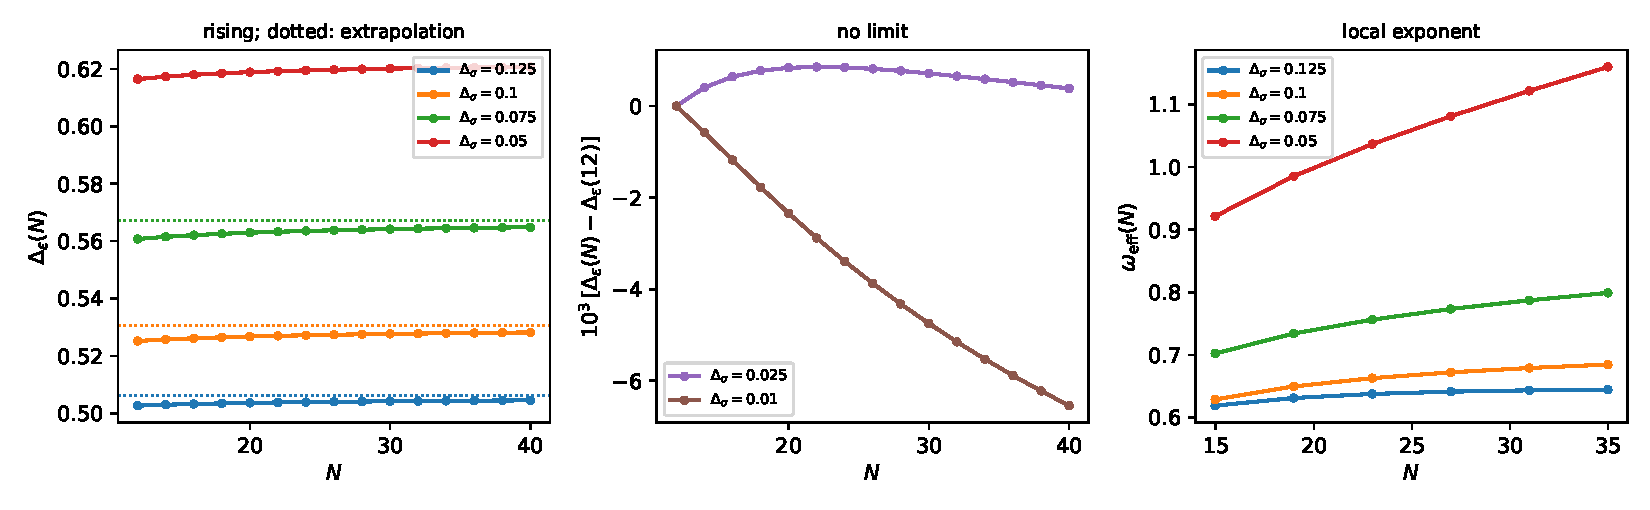
\includegraphics[width=\textwidth]{parts/ht/figures/fig_d1_cutoff.pdf}
\caption{$d=1$, \code{dens\_v1}.
\emph{Left:} $\DE(N)$ at $0.05\le\Ds\le0.125$; the dotted lines are the extrapolations of the stable series
(0.075 to 0.125).
\emph{Middle:} change $\DE(N)-\DE(12)$ at $\Ds=0.025$, which peaks near $N=\HTq{E8}$ and then falls, and at 0.01,
which falls at a nearly constant rate per unit of $\ln N$.
\emph{Right:} the local exponent~\eqref{ht:eq:omegaeff}, which levels off at 0.125 and 0.1 but rises at 0.075 and 0.05.}
\label{ht:fig:d1}
\end{figure}

\paragraph{Weak coupling and the $\eps$ expansion.}\label{ht:sec:d1-pert}
\begin{itemize}
\item At $\Ds=0.249$ the extrapolation differs from the $\eps$ series through $\eps^7$ (GFF folder:
 $C_2=(\pi+4\ln2)/9$, $C_3$ to $C_7$) by $\HTq{P1}$. That is below the $\HTq{P4}$ at which we trust the check,
 because of the series and fit systematics.
\item At $\Ds=0.24$ the value lies within the band $\HTq{P2}$ of the partial sums through $\eps^4$ to $\eps^7$.
\item The blind solver of Section~\ref{ht:sec:checks} computes the weak-coupling coefficient of the truncated model.
 With $\DE=\frac12-\frac\eps6+C_2(N)\eps^2+\dots$, it reproduces
 \begin{equation}
 C_2(N)=\frac{34}{81}+\sum_{n\ \text{even},\,2\le n\le N}v_n\Big[\frac{2}{81(n-\frac12)}+\frac{2}{9n}+\frac{2}{9(n+\frac12)}+\frac{2}{81(n+1)}\Big],\qquad v_n=\frac{(\frac12)_n}{n!},
 \label{ht:eq:C2N}
 \end{equation}
 to at most $3\times10^{-7}$ for $N=0$ to 16, raw and corrected. The limit of $C_2(N)$ is the GFF value; the
 approach is like $N^{-1/2}$.
\end{itemize}

\paragraph{Intermediate coupling.}
\begin{itemize}
\item The extrapolations are final for $\Ds\geq0.1$.
\item At $0.075\le\Ds\le0.125$ they add $\HTq{E7}$ to the $N=40$ values.
\item Over $15\le N\le35$ the local exponent levels off:
 \begin{itemize}
 \item at $\HTq{E1}$ for $\Ds=0.125$;
 \item at $\HTq{E2}$ for 0.1.
 \end{itemize}
\item It rises instead, over the same range of $N$:
 \begin{itemize}
 \item $\HTq{E3}$ at 0.075;
 \item $\HTq{E4}$ at 0.05.
 \end{itemize}
\item A rising $\omega_{\rm eff}$ precedes the turnover seen at $\Ds=0.025$ and suggests that the fits overestimate
 the limit. This is why 0.075 carries a one-sided error. The classification final versus one-sided is a judgement
 based on these trends; they differ only modestly between 0.1 and 0.075.
\item At weak coupling $\omega_{\rm eff}$ also rises slowly ($\HTq{E11}$ at $\Ds=0.249$), but the bias it implies is
 below $\HTq{E12}$.
\item Fits restricted to $N\le32$ predict $N=34$--40 to $\HTq{E5}$ (Table~\ref{ht:tab:d1-holdout}).
\end{itemize}

\begin{table}[t]
\centering\footnotesize\renewcommand{\arraystretch}{1.1}
\begin{tabular}{@{}l c c c c c c@{}}
\toprule
$\Ds$ & $\omega_{\rm eff}(15)$ & (19) & (23) & (27) & (31) & (35)\\
\midrule
\inputrows{parts/ht/sections/tab_d1_omegaeff.tex}
\bottomrule
\end{tabular}
\caption{Local exponent~\eqref{ht:eq:omegaeff} of the $d=1$ series, labelled by the centre of its four cutoffs.
Held-out test: fits on $N\le32$ predict the values at $N=34$--40 to within $\HTq{E5}$ at every $\Ds\ge0.05$, inside
the spread of the predictions. The test passes also at $\Ds=0.025$, where the series has no limit, so it checks the
fits only within the range of the data, not their limit. All values:
\code{results/HT\_1d/holdout\_and\_local\_exponent.md}.}
\label{ht:tab:d1-holdout}
\end{table}

\paragraph{Strong coupling.}
\begin{itemize}
\item \emph{$\Ds=0.05$.} The series still rises at $N=40$. The accepted F1 and F2 fits give $\HTq{D10}$, a range
 that contains the NRG value of Table~\ref{ht:tab:d1}. The F3 fits reach down to $\HTq{D11}$. Their low branch moves up as cutoffs are
 added, which mildly argues against a turnover.
 The rising $\omega_{\rm eff}$ argues the other way. No value is quoted.
\item \emph{$\Ds\le0.025$.} The corrected sequence does not converge.
 \begin{itemize}
 \item At 0.025 it peaks near $N=\HTq{E8}$ and then falls ever faster, reaching $\HTq{E9}$ per unit of $\ln N$ at
 $N=40$.
 \item At 0.01 it falls at a constant $\HTq{E10}$ per unit of $\ln N$.
 \item At 0.001 it falls slowly but lies $\HTq{C3}$ above the NRG value.
 \end{itemize}
 The zero-mode basis is converged and the solver is verified, so this is a property of the window model, not of the
 numerics. The uncorrected truncation converges, but to values that violate Eq.~\eqref{ht:eq:v}
 (Table~\ref{ht:tab:d1-ident}).
\end{itemize}

\subsection{Model dependence and the comparison with NRG}\label{ht:sec:d1-model}
The errors of Table~\ref{ht:tab:d1} are half-spreads of one family of fits (F1--F3) on one prescription. They do not cover two
further model dependences, which we measure on the shipped records
(\code{public/model\_dependence\_ht1d.py}, table in \code{results/HT\_1d/model\_dependence.md}).
\begin{itemize}
\item \emph{Tail model.} We tried two alternative descriptions of the approach $N\to\infty$ of the same window series:
 \begin{itemize}
 \item F4, Eq.~\eqref{ht:eq:fitN} with two free exponents;
 \item a local exponent continued linearly in $\ln N$ from its last four values, with the slope at $N=40$ integrated
 to infinity.
 \end{itemize}
 Both move the limit down by at most $\HTq{M3}$ at $0.075\le\Ds\le0.125$, of the order of the fit half-spread.
\item \emph{Prescription.} The same truncation without the window (raw, energy zero-mode basis) extrapolates, with
 the same fits, to limits $\HTq{M6}$ below the window limits at $\Ds=0.125$, 0.1 and 0.075, respectively.
 \begin{itemize}
 \item Neither prescription satisfies the descendant identities in the limit (Table~\ref{ht:tab:d1-ident}), so the
 limit of the truncated model depends on the prescription at this level.
 \item At $\Ds\ge0.15$ the two prescriptions agree to $\HTq{M7}$ or better.
 \end{itemize}
\end{itemize}
The prescription dependence, $\HTq{M10}$ at $0.075\le\Ds\le0.125$, is thus as large as the gap to NRG below. We do
not combine these shifts into an error. The truncation has no strict error bar, and an error built after the gap to
NRG had been seen would make the comparison read as agreement within errors. The errors of Table~\ref{ht:tab:d1} stay
the fit spreads. The window limit is expected to be the better of the two, since its $\sigma$ descendant violation is
$\HTq{V2}$ times smaller.

\paragraph{Comparison with NRG.} We compare with the final NRG values of Table~\ref{ht:tab:d1} (NRG folder). Their
errors are sums of three convergence diagnostics, not standard deviations.
\begin{itemize}
\item HT lies above NRG at all six points $0.075\le\Ds\le0.2$, by up to $\HTq{C1}$.
\item The differences are $\HTq{C5}$ to $\HTq{C1}$ at $0.075\le\Ds\le0.15$, and below $\HTq{C6}$ at 0.175 and 0.2.
\item At $\Ds=0.125$, 0.1 and 0.075 the differences are $\HTq{C2}$. They are at least five times both the fit
 half-spreads of Table~\ref{ht:tab:d1} and the NRG errors, and of the size of the prescription dependence.
\item NRG lies between the raw and the window limits at these three points.
\item NRG also lies inside the fit-free bracket $[\DE(40),\,\DE(40)+\frac{d\DE/d\ln N}{\omega_{\rm eff}}]$ of the
 window series at every $0.075\le\Ds\le0.2$. That bracket holds if $\DE(N)$ keeps rising and $\omega_{\rm eff}$
 does not decrease beyond $N=40$.
\end{itemize}
We do not assume that either method is right. The Monte Carlo values that the MC folder labels \emph{accepted}
(MC column of the $d=1$ results table of Ref.~\cite{ht:paper}) also lie above NRG at these three couplings, on the same side as HT, but their
systematic errors exceed the HT--NRG differences, so they cannot decide between the two. The resummed expansions cannot decide at this coupling
(\code{Resummation/} folder). The HT values at
$0.075\le\Ds\le0.125$ are limits of the window-corrected truncation at their fit errors. As estimates of the CFT
they depend on the truncation prescription by the shifts above, which are as large as the gap to NRG.

\subsection{Descendant identities}\label{ht:sec:d1-ident}
Table~\ref{ht:tab:d1-ident} gives the level-1 violations, Eq.~\eqref{ht:eq:v}, at $N=28$, raw and with the window, from
the identity diagnostic run on the \code{prod1--7} records. The other cutoffs are in
\code{results/HT\_1d/identity\_violations.md}.
\begin{itemize}
\item The raw violations do not decay with $N$ over $N=16$--28 and grow with the coupling. At $\Ds\le0.1$ they range
 over $\HTq{V1}$.
\item The window reduces the $\sigma$ violation by $\HTq{V2}$ times at $\Ds\le0.15$.
\item At $\eps\ge0.6$ non-decaying residuals of about $\HTq{V3}$ remain for $\sigma$ and $\phi^3$, and up to
 $\HTq{V4}$ for $\varepsilon$ at $\Ds\le0.05$.
\end{itemize}

\begin{table}[t]
\centering\footnotesize\renewcommand{\arraystretch}{1.1}
\begin{tabular}{@{}l r r r r r r@{}}
\toprule
 & \multicolumn{3}{c}{raw} & \multicolumn{3}{c}{window}\\
\cmidrule(lr){2-4}\cmidrule(l){5-7}
$\Ds$ & $\sigma$ & $\phi^3$ & $\varepsilon$ & $\sigma$ & $\phi^3$ & $\varepsilon$\\
\midrule
\inputrows{parts/ht/sections/tab_d1_ident.tex}
\bottomrule
\end{tabular}
\caption{Level-1 descendant violations $v_1$ at $N=28$, raw and with the consistent window, in the energy zero-mode
basis of \code{prod1--7}: $n_z=24$ at $\Ds\ge0.1$, 32 below. The $\varepsilon$ columns use the first excited
even state. $^a$:~ambiguous identification with the free $L_{-1}$. In the CFT all entries vanish.}
\label{ht:tab:d1-ident}
\end{table}

\IfFileExists{parts/ht/sections/d2/sec_d2.tex}{% sec_d2.tex -- d = 2 results of the finite-coupling HT note (from phi4HT2d, 2026-10-14; readability review 2026-10-15).
% Every number here has a replay row in repro_d2.tex / results_map.md (check names d2.*, i2.*).
% Needs: amsmath, booktabs, graphicx; macros \Ds, \DE, \eps, \ii, \code of the note. Inputs: tab_d2_values.tex,
% fig_d2_DeltaE.pdf (tools/make_d2_note_inputs.py, from HT/results/HT_2d/prod1/points.csv). Cites Sak:1973oqx, Behan:2017dwr, Behan:2017emf, Belavin:1984vu.
\section{Two dimensions}\label{ht:d2:sec}

\subsection{Modes, sectors and couplings}\label{ht:d2:modes}
In $d=2$ the exponent $s$ of the long-range interaction fixes $\Ds=(d-s)/2=1-s/2$, so $\eps=2s-2=2-4\Ds$. The
interacting window is $1<s<s_*$, that is $\frac18<\Ds<\frac12$. Its upper end is the crossover to the short-range Ising
CFT, at $s_*=2-\eta_{\rm SR}=\frac74$~\cite{ht:Sak:1973oqx,ht:Behan:2017dwr,ht:Behan:2017emf}. At $s=s_*$ the fixed point is the
short-range Ising CFT decoupled from a generalized free field~\cite{ht:Behan:2017dwr,ht:Behan:2017emf}, so there $\DE=1$, the
dimension of the energy operator of the two-dimensional Ising model~\cite{ht:Belavin:1984vu}. The scan covers
$\frac18\le\Ds<\frac12$.

The modes are $k=(a,b)$, $a,b\ge0$, of Eq.~\eqref{ht:eq:weights}: the oscillator $a_{ab}$ has level $\kappa=a+b$, spin
$j=a-b$ and weight $u_{ab}^2=(\Ds)_a(\Ds)_b/(a!\,b!)$. With $f_{ab}=e^{-\ii(a-b)\vartheta}$, the two-point function of
the field~\eqref{ht:eq:modes} is the cylinder covariance $z^{\Ds}|1-z\,e^{\ii\vartheta}|^{-2\Ds}$, with $z=e^{-\tau}$ the
radial-time variable and $\vartheta$ the angle on the circle. The oscillator $a_{00}$ is the zero mode of
Eq.~\eqref{ht:eq:split}, and all others form the bath. A bath state with occupations $n_{ab}$ has level, particle number
and spin
\begin{equation}
 \ell=\sum_{(a,b)\neq(0,0)}(a+b)\,n_{ab},\qquad P=\sum n_{ab},\qquad J=\sum(a-b)\,n_{ab}.
\end{equation}
We keep every bath state with $\ell\le N$, with no limit on $P$ (Section~\ref{ht:sec:split}). The scalar spectrum is
computed at $J=0$, in the sector even under the reflection $a\leftrightarrow b$. Since $\ell-J=2\sum b\,n_{ab}$ is
even, every scalar bath state has even level. The truncations at $N=2m$ and $2m+1$ therefore coincide, and we use the
even cutoffs $N=8,10,\dots,24$.

The vertices $W_j=\langle{:}\chi^j{:}\rangle$ of Eq.~\eqref{ht:eq:Hsplit} are built exactly in the retained scalar space.
With $B=\sum_{(a,b)\neq(0,0)}u_{ab}\,a_{ab}$ the annihilation part of $\chi$ at $\vartheta=0$, and $S$ the embedding of
the scalar space,
\begin{equation}
 W_j=\sum_{i=0}^{j}\binom ji\,(B^iS)^\dagger(B^{j-i}S).
 \label{ht:d2:eq:W}
\end{equation}
Between two scalar states the average over the circle equals the value at $\vartheta=0$, so no further projection is
needed; states of nonzero spin enter as intermediate states. Since $B$ lowers the level, $B^{j-i}S$ stays inside the
space $\ell\le N$, and the matrix elements are exact: no intermediate state is cut off.

The couplings are parametrized by $\theta=(\theta_0,\theta_1)$,
\begin{equation}
 g=\frac{192\,e^{3\theta_1}}{\Ds^2},\qquad A=\frac{4\,e^{2\theta_1}\theta_0}{\Ds},\qquad
 r=A+\frac g2-\frac{\Ds}4 ,
 \label{ht:d2:eq:theta}
\end{equation}
with $A$ the coefficient of $q^2$ in $H_z$, Eq.~\eqref{ht:eq:Hz}. The two tuning conditions of Eq.~\eqref{ht:eq:tune},
$E_\sigma-E_v=\Ds$ and $E_{\phi^3}-E_v=2-\Ds$, fix $\theta$, and the prediction is $\DE=E_\varepsilon-E_v$.

\subsection{Zero-mode basis and window}\label{ht:d2:basis}
The zero-mode basis is the density basis of Section~\ref{ht:sec:zerobasis}, Eq.~\eqref{ht:eq:rho}, with the training cutoff
$N_t=6$. The teacher is an energy-basis calculation at $N=6$ with 24 states per parity, taken from an auxiliary
oscillator basis of $N_{\rm osc}=192$ states. Each stored basis keeps the 20 leading eigenvectors of $\rho$ per parity,
which contain the nested bases of $n_z=12$, 16 and 20 states. Production uses $n_z=16$, and $n_z=20$ and 12 are
recomputed at every cutoff as checks. For ten values of $\Ds$ the stored bases are those of the package; for
$\Ds=0.125$, 0.135 and 0.175 new ones were trained with the same settings. No basis is transferred between values of
$\Ds$. Over all chains and cutoffs,
\begin{equation*}
 |\DE(n_z{=}20)-\DE(n_z{=}16)|\le9.4\times10^{-11},\qquad |\DE(n_z{=}12)-\DE(n_z{=}16)|\le5.2\times10^{-7},
\end{equation*}
the latter at $\Ds=0.125$, $N=22$. Three reference points at $N=14$ ($\Ds=0.126$, 0.25 and 0.4) use instead the energy
basis with 32 states per parity, recomputed at every coupling from $N_{\rm osc}=256$; they agree with $n_z=16$ to
$10^{-9}$.

The window is the consistent correction of Section~\ref{ht:sec:window}, Eqs.~\eqref{ht:eq:window} and~\eqref{ht:eq:Ev}. Every
bath state of level $\ell$ is shifted by $D(\ell)=E_v(N)-E_v(N-\ell)$. The vacua $E_v(M)$, $M=0,2,\dots,N$, are computed
with their own windows, at the same couplings and in the same zero-mode basis; they are not retuned. Their fixed points
are solved as in Section~\ref{ht:sec:window} and accepted at $10^{-11}$, and the derivatives~\eqref{ht:eq:dEv} enter the
tuning Jacobian. The other acceptance thresholds are a tuning residual $\le1.5\times10^{-10}$, an eigenvector residual
$\le10^{-8}$ and an orthogonality defect $\le10^{-9}$. Every shipped record passes them (check \code{d2.records.gates}).

\subsection{Campaign}\label{ht:d2:campaign}
Thirteen chains, $\Ds\in\{0.125,0.126,0.135,0.15,0.175,0.2,0.25,0.3,0.35,0.4,0.45,0.475,0.495\}$, ran from $N=8$ to 24
in steps of two on Expanse (SDSC), one chain per 64-core, 64\,GB allocation. Each cutoff was seeded by the previous one,
and the first by the package's $N=8$ reference solution or by the teacher. The 348 records (main runs, basis checks and
reference points) took $1.1\times10^4$ core-hours; a point at $N=24$ took 0.6--11\,h and up to 24\,GiB. The code is
\code{lri\_2d\_window\_hpc} at commit 889a968, and every record carries a hash of that source. The Python environment
was frozen (Python 3.11.5, NumPy 2.3.5, SciPy 1.17.0, Numba 0.65.1). The lowest value, $\Ds=0.125$, is the crossover
point $s=s_*$, where $\DE=1$.

\subsection{Finite-cutoff behaviour}\label{ht:d2:finiteN}
Table~\ref{ht:d2:tab:values} and Fig.~\ref{ht:d2:fig:DE} give $\DE(N)$. All of them are values of the truncated model at that
cutoff (status: \emph{finite-$N$}). Nine cutoffs up to $N=24$ are too few, and the behaviour varies too much with $\Ds$,
for a controlled extrapolation, so we quote no continuum value in $d=2$. Steps are taken between successive cutoffs,
$\delta(N)=\DE(N)-\DE(N-2)$.
\begin{itemize}
\item $\Ds\ge0.45$: the last step $\delta(24)$ is $2.54\times10^{-6}$, $1.28\times10^{-6}$ and $1.57\times10^{-7}$ at
 0.45, 0.475 and 0.495, and the steps shrink by 18--22\% per step.
\item $0.25\le\Ds\le0.4$: $\DE$ rises monotonically, with last steps $4.30\times10^{-4}$, $3.80\times10^{-4}$,
 $2.16\times10^{-4}$ and $5.86\times10^{-5}$, which shrink by $1-(\delta(24)/\delta(16))^{1/4}=16$, 13, 11 and 8\% per
 step. If the rise continues, $\DE(24)$ bounds the limit of the truncated model from below.
\item $\Ds=0.2$: the steps change sign ($+$ up to $N=22$, $-4.2\times10^{-5}$ at $N=24$), so $\DE$ is not monotone.
\item $0.125\le\Ds\le0.175$: $\DE$ falls from $N=10$ on, and the steps grow. The last step is $-1.05\times10^{-3}$ at
 0.175 ($N=24$) and $-2.02\times10^{-2}$ at 0.125 ($N=22$), each larger than the previous one. At $\Ds=0.125$ the value
 at $N=22$, 0.9400, lies $6\%$ below the exact value 1 and moves away from it. This is the failure toward the
 short-range end discussed in Section~\ref{ht:d2:caveats}.
\end{itemize}

\subsection{No solution at \texorpdfstring{$N=24$}{N=24} for \texorpdfstring{$\Ds=0.125$, 0.126}{small Delta sigma}: a fold}\label{ht:d2:fold}
At $\Ds=0.125$ and 0.126 the Newton solve at $N=24$ did not converge. It was started from the $N=22$ root and from the
linear extrapolation $2\theta(22)-\theta(20)$, and repeated with a finite-difference Jacobian. Each time the residual
stalled on a floor, at $2.9\times10^{-3}$ and $2.0\times10^{-3}$. At the accepted roots of smaller $N$ the condition
number of the tuning Jacobian grows, from 84 at $N=12$ to 888 at $N=22$ ($\Ds=0.125$).

To decide whether a root exists, we scanned the valley of the residual. Write the conditions as
\begin{equation}
 f_1(\theta)=E_\sigma-E_v-\Ds,\qquad f_2(\theta)=E_{\phi^3}-E_v-(2-\Ds).
\end{equation}
At six values $\theta_0\in\{12.5,13.25,\theta_0^{\rm best},14.3,14.8,15.5\}$ around the best point of the Newton solves,
a secant iteration in $\theta_1$ solves $f_2=0$ to $|f_2|\le10^{-9}$, and we record $f_1$ there. Code, basis and solver
settings are those of production, with $n_z=16$. At $\theta_0^{\rm best}$ the first evaluation, before the secant,
reproduces the stalled residual: $\max(|f_1|,|f_2|)=2.93\times10^{-3}$ and $1.99\times10^{-3}$. A root would show as a
sign change of $f_1$ along the curve $f_2=0$. There is none: $f_1>0$ at every point (smallest value
$1.60\times10^{-3}$), with an interior minimum and a steep rise on both sides. A quartic fit in $\theta_0$ puts the
minimum at $f_1=2.686\times10^{-3}$ ($\theta_0\approx14.03$) for $\Ds=0.125$ and at $1.556\times10^{-3}$
($\theta_0\approx14.06$) for 0.126. Both are far above the effect of the zero-mode truncation ($\le5\times10^{-7}$) and
the eigensolver accuracy.

Hence, on the scanned range of $\theta_0$, the two tuning conditions have no solution at $N=24$ on the branch continued
from smaller $N$. This is a statement about the truncated model at $N=24$ and involves no extrapolation in $N$. The
minimum falls by $1.13\times10^{-3}$ per $0.001$ in $\Ds$. Near a saddle-node (fold) it is linear in the parameter,
which places the fold at
\begin{equation}
 \Ds^{\rm fold}(N=24)\approx0.1274,
\end{equation}
an estimate from two values of $\Ds$. Roots exist above it ($\Ds=0.135$ converged at $N=24$), and at $N=22$ they exist
down to 0.125. The fold has therefore moved past 0.125 between $N=22$ and 24, and the growing condition number at the
roots is its precursor. The $d=2$ data at $\Ds=0.125$ and 0.126 end at $N=22$.

\subsection{Weak coupling and the \texorpdfstring{$\epsilon$}{epsilon} expansion of the model}\label{ht:d2:weak}
Expanded in $\eps$, the truncated model agrees with the consistent-window scheme of the perturbative calculation
(\code{HT\_Pert/}). At $\Ds=0.495$ ($\eps=0.02$) the $[4/4]$ Pad\'e approximant of that scheme's coefficients
$C_0(N),\dots,C_8(N)$ reproduces $\DE(N)$ to $9.4\times10^{-12}$ at every $N=8,\dots,24$, and at $\Ds=0.475$
($\eps=0.1$) to $7.6\times10^{-8}$ (check \code{d2.pert\_consistent}). A difference $\delta C_4$ in the fourth-order
coefficient would show as $\delta C_4\,\eps^4$, so $|\delta C_4|\lesssim6\times10^{-5}$ at every $N\le24$. In that
scheme the fourth-order coefficient grows with the cutoff, $C_4(N)\simeq5.003-\frac{365}{4374\pi}\ln N$, that is like
$-0.027\ln N$ (exact sums to $N=2000$ in \code{HT\_Pert/}), while the continuum value $C_4(2)$ is finite. The $d=2$
window model is thus known to be correct only through third order in $\eps$. In the perturbative calculation a larger
correction, the complete window of \code{HT\_Pert/}, removes this logarithm; it has no finite-coupling counterpart here.

\begin{table}[t]
\centering\small\setlength{\tabcolsep}{4.5pt}
\begin{tabular}{@{}l l l l l l l l@{}}
\toprule
$\Delta_\sigma$ & $s$ & $N=16$ & $N=20$ & $N=22$ & $N=24$ & last step & behaviour\\
\midrule
0.125 & 1.75 & 0.98916082 & 0.96025057 & 0.94002832 & n.s. & $-2.02\times10^{-2}$ & falls; steps grow\\
0.126 & 1.748 & 0.99053540 & 0.96363343 & 0.94568294 & n.s. & $-1.80\times10^{-2}$ & falls; steps grow\\
0.135 & 1.73 & 0.99948557 & 0.98399079 & 0.97537120 & 0.96202900 & $-1.33\times10^{-2}$ & falls; steps grow\\
0.15 & 1.7 & 1.00548133 & 0.99836315 & 0.99471461 & 0.99022622 & $-4.49\times10^{-3}$ & falls; steps grow\\
0.175 & 1.65 & 1.00330217 & 1.00162583 & 1.00076308 & 0.99971675 & $-1.05\times10^{-3}$ & falls; steps grow\\
0.2 & 1.6 & 0.99490861 & 0.99526003 & 0.99534664 & 0.99530455 & $-4.21\times10^{-5}$ & not monotone\\
0.25 & 1.5 & 0.97541470 & 0.97674862 & 0.97727730 & 0.97770747 & $+4.30\times10^{-4}$ & rises; shrink 16\%/step\\
0.3 & 1.4 & 0.96158682 & 0.96267180 & 0.96311194 & 0.96349241 & $+3.80\times10^{-4}$ & rises; shrink 13\%/step\\
0.35 & 1.3 & 0.95679429 & 0.95736832 & 0.95760910 & 0.95782471 & $+2.16\times10^{-4}$ & rises; shrink 11\%/step\\
0.4 & 1.2 & 0.96152920 & 0.96167002 & 0.96173269 & 0.96179129 & $+5.86\times10^{-5}$ & rises; shrink 8\%/step\\
0.45 & 1.1 & 0.97526784 & 0.97527566 & 0.97527858 & 0.97528111 & $+2.54\times10^{-6}$ & small steps\\
0.475 & 1.05 & 0.98580651 & 0.98581110 & 0.98581268 & 0.98581396 & $+1.28\times10^{-6}$ & small steps\\
0.495 & 1.01 & 0.99678104 & 0.99678155 & 0.99678174 & 0.99678190 & $+1.57\times10^{-7}$ & small steps\\
\bottomrule
\end{tabular}

\caption{$\DE(N)$ in $d=2$ at finite coupling ($n_z=16$, consistent window): finite-$N$ values of the truncated model,
not continuum values. n.s.: no solution at $N=24$ (Section~\ref{ht:d2:fold}). Last step: between the two largest cutoffs.
Shrink: $1-(\delta(24)/\delta(16))^{1/4}$.}
\label{ht:d2:tab:values}
\end{table}

\begin{figure}[t]
\centering
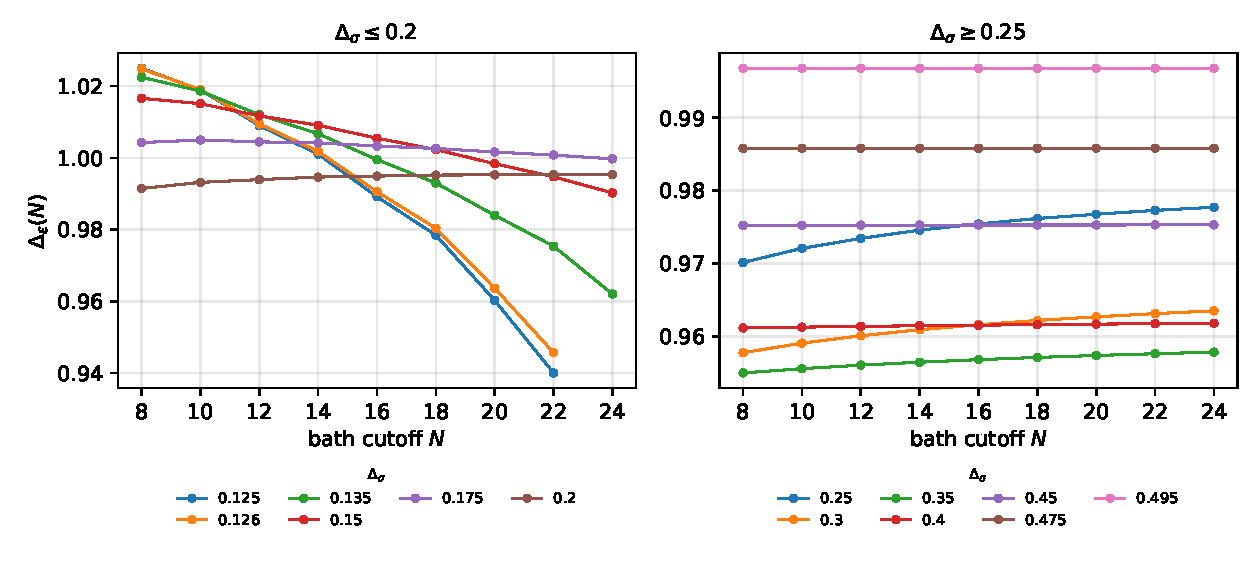
\includegraphics[width=\textwidth]{parts/ht/sections/d2/fig_d2_DeltaE.pdf}
\caption{$\DE(N)$ in $d=2$ against the bath cutoff $N$, for the 13 values of $\Ds$ (made by
\code{tools/make\_d2\_note\_inputs.py} from \code{HT/results/HT\_2d/prod1/points.csv}).}
\label{ht:d2:fig:DE}
\end{figure}
}{%
\section{Two dimensions}\label{ht:d2:sec}
\textit{Section to be supplied by the $d=2$ contributors (phi4HT2d): modes and weights, the $d=2$ window, campaigns
($N\le24$), finite-$N$ results with status words, the fold near $\Ds\approx0.1274$. Pending
the transfer of the production records from Expanse.}}

% d = 3 results section for the HT note (phi4HT3d, 2026-10-13; readability review 2026-10-15). Every number carries
% the check id of `make replay` (HT/code/lri_3d_window_hpc or lri_3d_window_indep) in a comment; see repro_d3.tex.
% Uses amsmath, booktabs, graphicx and the note's \code. Inputs tab_d3_finiteN.tex (generated by public/note_d3.py)
% and fig_d3_steps.pdf.
\section{Three dimensions}\label{ht:d3:sec}

\subsection{Modes, sectors and the truncated space}\label{ht:d3:modes}

On $S^2\times\mathbb R$ of unit radius we use the modes $k=(n,l,m)$ of Eq.~\eqref{ht:eq:weights}, with $n,l\geq0$ and
$|m|\leq l$, level $\kappa=2n+l$ and energy $\Delta_\sigma+\kappa$. With $z=e^{-\tau}$ and $\mu$ the cosine of the
angle between the two points, the two-point function of the generalized free field is
\begin{equation}
 \frac{z^{\Delta_\sigma}}{(1-2z\mu+z^2)^{\Delta_\sigma}}=\sum_{\kappa\geq0}z^{\Delta_\sigma+\kappa}\,G_\kappa(\mu),\qquad
 G_\kappa(\mu)=\sum_{2n+l=\kappa}(2l+1)\,u_{nl}^2\,P_l(\mu).
 \label{ht:d3:weights}
\end{equation}
Here $G_\kappa=C_\kappa^{(\Delta_\sigma)}$ is the Gegenbauer polynomial, written $G$ to avoid a clash with the
coefficients $C_n$, and $P_l$ is the Legendre polynomial. Expanding $G_\kappa$ in Legendre polynomials fixes the
weights $u_{nl}^2$ of Eq.~\eqref{ht:eq:weights}. The zero mode $k=(0,0,0)$ has $u=1$; it is the oscillator $a_0$ of
Eq.~\eqref{ht:eq:split}, with coordinate $q$. The bath field is
$\chi=\sum_{k\neq(0,0,0)}u_{nl}\sqrt{4\pi}\,\big[Y_{lm}\,a_k+\text{h.c.}\big]$, and sphere averages use
$d\Omega/4\pi$. A bath state with occupation numbers $n_k$ has level $\ell=\sum_k\kappa_k n_k$. We keep all states
with $\ell\leq N$, with no limit on the particle number.

\textit{Sectors.} Rotations, inversion $(-1)^\ell$ and field parity commute with $H$. The scalar operators live in
the $J=0$, inversion-even sector, in both field parities. Inversion-even states have even $\ell$, so an odd cutoff
adds no scalar state, and we use even $N$ only. The $J=0$ subspace is the kernel of $J_+$ within the $J_z=0$
subspace. It is built separately in every species-occupation block, a species being $(n,l)$ with its $2l+1$ magnetic
states, and it is computed as an SVD null space.

At $N\geq18$ LAPACK's default SVD driver (gesdd) fails to converge on a few blocks. The code then retries with the
gesvd driver and full right singular vectors. It accepts the kernel $Q$ only if its dimension is the nullity
predicted by representation theory and if every matrix element of $J_+Q$ and of $Q^{\mathsf T}Q-1$ is at most
$10^{-10}$ in absolute value; a second failure is an error. The retry happened in 8 of 17\,335 blocks at $N=18$ and
in 62 of 40\,033 at $N=20$, with $\max|J_+Q|=5.8\times10^{-15}$ % PROJECTOR
(it does not depend on $\Delta_\sigma$). The scalar bath space has 110, 371, 1285, 4486, 15\,815, 55\,859 and
196\,585 states at $N=8,10,\dots,20$; % SIZE
with $n_z=16$ zero-mode states per parity, the scalar problem at $N=20$ has dimension $3.1\times10^6$ in each field
parity.

\textit{Vertices.} The couplings $W_j=\langle{:}\chi^j{:}\rangle$ of Eq.~\eqref{ht:eq:Hsplit}, restricted to $J=0$,
equal the vertex at any single point of the sphere, by rotation invariance. The code evaluates them at the north
pole. The $J=1$ and $J=2$ sectors are computed only as diagnostics; there the code uses the trace over the $2J+1$
magnetic components, and the original polar Gauss--Legendre quadrature (with $N+1$ nodes) is kept as an independent
test. The vertices at lower cutoffs, which the window needs, are exact restrictions of those at $N$, because a
normal-ordered $W_j$ never passes through a level above both of its endpoints.

\subsection{Window, zero-mode basis and tuning}\label{ht:d3:window}

The window of Eq.~\eqref{ht:eq:window} is used in its self-consistent form. Only even sub-cutoffs carry distinct
vacua, so a bath state of level $\ell$ is shifted by
\begin{equation}
 D_N(\ell)=E_v(N)-E_v\big(2\lfloor(N-\ell)/2\rfloor\big),\qquad E_v(M)=\lambda_{\min}\big[H(M)+D_M\big],\quad E_v(0)=0 ,
 \label{ht:d3:window-floor}
\end{equation}
with $E_v(M)$ the lowest field-even scalar energy at sub-cutoff $M$, solved one sub-cutoff after the other. At each
sub-cutoff the fixed point $v=E_v(M)$ solves $F(v)=\lambda_{\min}[H(M)+D(v)]-v=0$. Newton's method converges on it
because $F'(v)=-p_0$, with $p_0$ the bath-vacuum weight of the ground state. The iteration stops when
$|F|\leq\min\big(10^{-12}\max(1,|v|),\,10^{-11}\big)$ and fails if $p_0\leq10^{-12}$. The same $D_N$ is applied,
without retuning, in the $J=1,2$ sectors.

The zero-mode basis is the density basis of Section~\ref{ht:sec:zerobasis}, trained once per $\Delta_\sigma$. The teacher
is a solve at $N_t=6$ in the energy basis, with 24 states per parity taken from an auxiliary oscillator basis of
$N_{\rm osc}=192$ states. The reduced density matrix of Eq.~\eqref{ht:eq:rho} is then
$(\rho_{\rm vac}+\rho_\sigma+\rho_{\phi^3})/6$ at $N_t$ plus the vacua at $M=0,2,4$, each with weight $1/6$. The stored
basis keeps its 20 leading eigenvectors per parity, and every production solve at $N=8,\dots,20$ uses the leading
$n_z=16$. % CONFIG
As in $d=1$, the $\varepsilon$ state plays no role in the training.

The couplings $(r,g)$ are tuned by Eq.~\eqref{ht:eq:tune}, $E_\sigma-E_v=\Delta_\sigma$ and
$E_{\phi^3}-E_v=3-\Delta_\sigma$, by safeguarded Newton steps with tolerance $3\times10^{-11}$. Each cutoff is started
from the solution at $N-2$, with the same zero-mode basis. A point is accepted only if
\begin{itemize}
\item both tuning conditions hold to $1.5\times10^{-10}$ (five times the Newton tolerance);
\item the eigenvector residuals are at most $10^{-8}$ and their orthogonality defects at most $10^{-9}$;
\item every window fixed point holds to $10^{-11}$. % REC-RECORDS
\end{itemize}
The replay also checks that the two tuned gaps of every record equal their targets to $10^{-9}$. The prediction is
$\Delta_\varepsilon=E_\varepsilon-E_v$, the first excited field-even scalar gap.

\subsection{Campaigns}\label{ht:d3:campaigns}

We solve 15 values of $\Delta_\sigma$: 0.7499, 0.745, 0.74, 0.725, 0.7, 0.675, 0.65, 0.625, 0.6, 0.575, 0.55, 0.535,
0.525, 0.52 and 0.518149. The last lies $1.9\times10^{-7}$ above the $\Delta_\sigma$ of the 3d Ising
model~\cite{ht:Chang:2024whx}, which is not imposed. Each value is computed as one sequence of solves, the teacher at
$N=6$ followed by $N=8,10,\dots,20$, each started from the previous one. Everything ran on SDSC Expanse (AMD EPYC
7742). Before production, each installed code release had to pass a validation job, the test suite and validators
that \code{make test} runs. Every step then ran with the arguments fixed in advance in a campaign manifest
(\code{code/lri\_3d\_window\_hpc/public/PROVENANCE.md}).

The records are grouped in five campaigns, which name the folders of \code{data/HT\_3d/campaigns}:
\begin{itemize}
\item \code{grid18} ($\Delta_\sigma\geq0.52$, 14 values) and \code{grid18sri} ($\Delta_\sigma=0.518149$, near the
 short-range Ising end): the teacher and $N=8$ to 18. Each sequence used 16 cores. A point at $N=18$, with $J=1$
 diagnostics, took 34--74 minutes at a peak of 38.5\,GiB. % COST-L18
\item \code{l20x06} ($\Delta_\sigma=0.6$, with $J=1$ diagnostics), \code{grid20} (the other 13 values
 $\Delta_\sigma\geq0.52$) and \code{grid20sri} ($\Delta_\sigma=0.518149$): $N=20$, the last two in the scalar sector
 only. The bath graph and the scalar projector do not depend on $\Delta_\sigma$, so they were built once into a cache
 that is never modified afterwards. On one large-memory node this took 9.0\,h and 92\,GiB, mostly in single-threaded
 LAPACK (from the Slurm log of a setup run, not a shipped record). The vertices depend on $\Delta_\sigma$ and are
 built in every point. A scalar-only point took 27--104 minutes at 84--87\,GiB on 32 cores; the point at
 $\Delta_\sigma=0.6$ with $J=1$ diagnostics took 239 minutes at 328\,GiB. % COST-L20
\end{itemize}

$N=22$ was not attempted.

\subsection{Results}\label{ht:d3:results}

Table~\ref{ht:d3:tab-finiteN} gives $\Delta_\varepsilon(N)$ at $N=14$--20; all of $N=8$--20 is in
\code{results/HT\_3d/finite\_L\_table.csv} (check \texttt{TABLE}). Figure~\ref{ht:d3:fig-steps} shows the steps
$d_N=\Delta_\varepsilon(N)-\Delta_\varepsilon(N-2)$. We reach $N=20$ at every $\Delta_\sigma$ % NMAX
and give finite-$N$ values only. These cutoffs are too few for a controlled extrapolation, and the checks below
show that small steps do not imply convergence.

\begin{table}[h]
\centering
\footnotesize
\begin{tabular}{@{}l llll r r@{}}
\toprule
$\Delta_\sigma$ & $N=14$ & $N=16$ & $N=18$ & $N=20$ & $d_{20}$ & $d_{20}/d_{18}$\\
\midrule
0.7499 & 1.49993336 & 1.49993336 & 1.49993336 & 1.49993336 & $2.3\times10^{-11}$ & 0.78\\
0.745 & 1.49673611 & 1.49673617 & 1.49673622 & 1.49673626 & $3.7\times10^{-8}$ & 0.75\\
0.74 & 1.49360198 & 1.49360214 & 1.49360225 & 1.49360232 & $7.3\times10^{-8}$ & 0.68\\
0.725 & 1.48486049 & 1.48485983 & 1.48485909 & 1.48485833 & $-7.6\times10^{-7}$ & 1.03\\
0.7 & 1.47194111 & 1.47193446 & 1.47192895 & 1.47192480 & $-4.2\times10^{-6}$ & 0.75\\
0.675 & 1.46046754 & 1.46048280 & 1.46050270 & 1.46052707 & $2.4\times10^{-5}$ & 1.23\\
0.65 & 1.45028710 & 1.45039728 & 1.45050697 & 1.45061574 & $1.1\times10^{-4}$ & 0.99\\
0.625 & 1.44146308 & 1.44172312 & 1.44196302 & 1.44218479 & $2.2\times10^{-4}$ & 0.92\\
0.6 & 1.43396549 & 1.43439430 & 1.43477460 & 1.43511242 & $3.4\times10^{-4}$ & 0.89\\
0.575 & 1.42767821 & 1.42827172 & 1.42878594 & 1.42922982 & $4.4\times10^{-4}$ & 0.86\\
0.55 & 1.42244491 & 1.42318494 & 1.42381704 & 1.42434921 & $5.3\times10^{-4}$ & 0.84\\
0.535 & 1.41973557 & 1.42054979 & 1.42124152 & 1.42181519 & $5.7\times10^{-4}$ & 0.83\\
0.525 & 1.41808151 & 1.41893773 & 1.41966339 & 1.42025885 & $6.0\times10^{-4}$ & 0.82\\
0.52 & 1.41729470 & 1.41816931 & 1.41890994 & 1.41951431 & $6.0\times10^{-4}$ & 0.82\\
0.518149 & 1.41700967 & 1.41789062 & 1.41863643 & 1.41924372 & $6.1\times10^{-4}$ & 0.81\\
\bottomrule
\end{tabular}

\caption{$\Delta_\varepsilon$ from the $d=3$ window truncation at bath cutoffs $N=14$--20, with the last step
$d_{20}=\Delta_\varepsilon(20)-\Delta_\varepsilon(18)$ and its ratio to the previous one. Finite-cutoff values, not
limits.}
\label{ht:d3:tab-finiteN}
\end{table}

\begin{figure}[h]
\centering
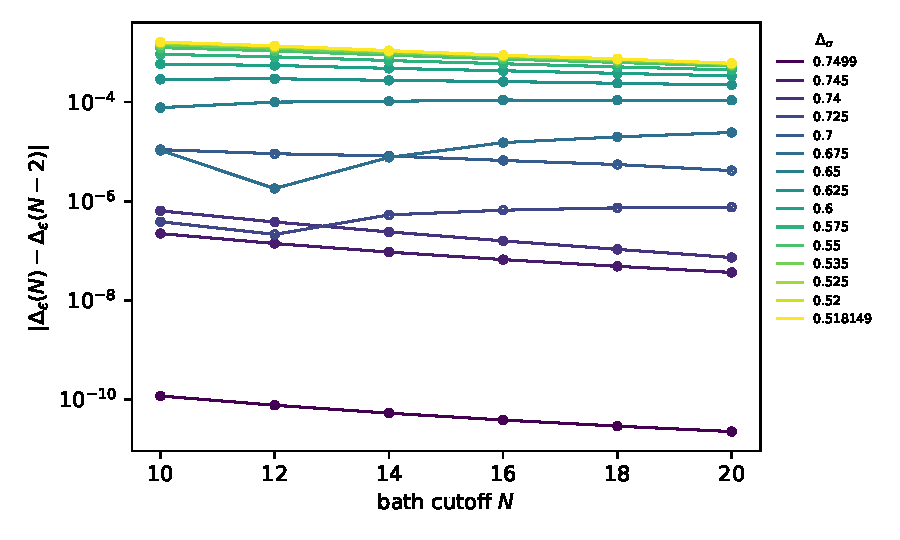
\includegraphics[width=0.75\textwidth]{parts/ht/sections/d3/fig_d3_steps.pdf}
\caption{Size of the steps $d_N$ against $N$, for every $\Delta_\sigma$; filled symbols: $d_N>0$, open: $d_N<0$.
Made by \code{public/note\_d3.py} from \code{finite\_L\_table.csv}.}
\label{ht:d3:fig-steps}
\end{figure}

\begin{itemize}
\item \textit{Weak coupling, $\Delta_\sigma\geq0.74$: small steps.} The last step is below $10^{-7}$
 ($7.3\times10^{-8}$ at most). % CONV-STEP
\item \textit{$\Delta_\sigma=0.7$: not converged, and moving away.} The Borel--Pad\'e resummation of the
 $\epsilon$ series through the GFF coefficient $C_7(3)$~\cite{ht:paper} fixes the continuum value to $1.47214(3)$. This is
 the median and half-spread of 29 approximants, with Borel--Leroy $b=0,\dots,4$ and Pad\'e orders of total degree 4
 and 5, rejecting those with a pole on the positive axis. % BP-0.7
 The value at $N=20$, $1.4719248$, lies $2.2\times10^{-4}$ below it, and the sequence
 $\Delta_\varepsilon(16)>\Delta_\varepsilon(18)>\Delta_\varepsilon(20)$ moves away. % BP-DEV
 The continuum is reached, if at all, only after a turnover at larger $N$. An extrapolation in $N$ that
 continues this trend lands below $\Delta_\varepsilon(20)$, further from the continuum, so none is quoted.
\item \textit{$\Delta_\sigma=0.65$ and $0.675$: no trend yet.} The steps do not yet shrink: $d_{20}/d_{18}=0.99$
 and 1.23. % NO-SHRINK
 At 0.7 and 0.725 the values fall (last steps $-4.2\times10^{-6}$ and $-7.6\times10^{-7}$), and from 0.675 down
 they rise, so the steps change sign in this range.
\item \textit{$0.518\leq\Delta_\sigma\leq0.625$: rising.} The values rise monotonically from $N=8$ to 20. % MONO-RISE
 The last steps are $(2.2\text{--}6.1)\times10^{-4}$, % MONO-STEPS
 and they shrink by 8 to 19 percent per step. % MONO-SHRINK
 They shrink fastest near the short-range end.
\item \textit{Short-range end, $\Delta_\sigma=0.518149$: fails near the endpoint.} The value at $N=20$,
 $1.41924$, lies above the 3d Ising value $\Delta_\varepsilon=1.41263$~\cite{ht:Chang:2024whx} and still rises. % SR-L20
 Near this end the long-range model is described by the short-range Ising model coupled, through its spin field, to
 an auxiliary generalized free field~\cite{ht:Behan:2017dwr,ht:Behan:2017emf}. That coupling is nearly marginal here, and
 the approach to the limit is expected to be logarithmic in $N$.
\item \textit{The window model at fourth order: a finite-$N$ statement.} Expanded in $\epsilon$ at fixed $N$, the
 same window model has $C_2(N)\to C_2(3)$, and $C_3(N)$ is consistent with $C_3(3)$ (\code{HT\_Pert/}). Its
 fourth-order coefficient at $N=20$, $0.7400078$, is 60\% of $C_4(3)=1.228063545$~\cite{ht:paper} and still growing
 slowly with $N$; whether its $N\to\infty$ limit is wrong is not shown. % C4-RATIO
\end{itemize}

The $N=20$ values are the $d=3$ Hamiltonian-truncation results of Ref.~\cite{ht:paper}: rounded to five decimals in its
$d=3$ results table, and plotted as green squares in the right panel of its comparison figure. % NUM3


\section{Independent checks}\label{ht:sec:checks}
In each dimension a second solver, written without using the production code, reproduces the production spectra at
finite cutoff. These checks verify that we compute the stated model, not that its limit is the CFT.

\paragraph{One dimension.}\label{ht:d1:checks}
\begin{itemize}
\item \emph{Authorship.} A Claude Code subagent wrote the solver (\code{code/lri\_dressed\_phi4\_independent\_check})
 from the definition of the model. It was not allowed to read the production code, results or analysis. Of the
 package documentation it read only the definition of the window (\code{docs/WINDOW.md}) and of the Hamiltonian
 (\code{docs/ALGORITHM.md}). It derived $H$ itself from the GFF radial
 quantization, and its derivation agrees with Eqs.~\eqref{ht:eq:Hz}--\eqref{ht:eq:Lj}.
\item \emph{Own numerics.} The zero mode is a sinc discrete-variable representation, the bath Fock space is its own,
 and both the literal and consistent windows are implemented. Newton tuning continues from weak coupling. Every point
 is verified on 1.5 times finer and 1.5 times wider grids.
\item \emph{Comparison set.} 38 points: raw and consistent at $\Ds=0.249$, 0.2, 0.1, 0.05, 0.025 and 0.01 with
 $N=12$, 16 and 20, plus literal at 0.2 and 0.1 with $N=12$.
\item \emph{Agreement with the production records} (\code{dens\_v1}, density basis, $n_z=16$). At the 18
 consistent-window points ($N=12$, 16, 20) the records agree with the blind solver to $5.6\times10^{-7}$ or better,
 the truncation error of the density basis.
\item \emph{Agreement with the energy-basis records} (\code{prod1--7}).
 \begin{itemize}
 \item $\DE$ agrees to $1.3\times10^{-9}$ where these records used $n_z=48$ or $\Ds\ge0.2$.
 \item It agrees to $4.8\times10^{-9}$ where they used $n_z=24$ or 32 at strong coupling, which is that basis's
 truncation error.
 \item Over all 38 points this gives $5\times10^{-9}$. The other levels and the tuned $(g,r)$ agree at the same level.
 \end{itemize}
\item \emph{Weak coupling.} The solver reproduces $C_2(N)$, Eq.~\eqref{ht:eq:C2N}, to $3\times10^{-7}$. It also shows
 that the window changes $\DE$ only at order $\eps^4$: the fitted exponent is 4.05 to 4.11.
\end{itemize}

% checks_d2.tex -- d = 2 paragraph of the independent-checks section (from phi4HT2d, 2026-10-14; review 2026-10-15).
% Checks i2.*, d2.*.
\paragraph{Two dimensions.}\label{ht:d2:checks}
A second solver, \code{lri\_2d\_window\_indep}, implements the $d=2$ model of Section~\ref{ht:d2:modes} from its written
definition, without using the production code. Its numerics differ:
\begin{itemize}
\item bath vertices from explicit annihilation amplitudes, on a dictionary representation of the Fock states;
\item reflection-even states as explicit symmetric combinations;
\item the zero mode in the energy basis, the lowest eigenstates of $H_z$ with $K$ states per parity, instead of the
 density basis;
\item its own Newton iteration for the window fixed points, and tuning by a finite-difference Newton method.
\end{itemize}
It is not blind: its author had earlier prepared the production code for the cluster. Its self-tests compare the
vertices with a brute-force construction in the full Fock space at $N=5$, and its Lanczos solver with dense
diagonalization. At the production couplings it reproduces the production spectra (155 runs at 13 values of $\Ds$; each
comparison is bound to the shipped record by its hash):
\begin{itemize}
\item With a converged zero-mode basis ($K\ge32$) it reproduces $\DE$ to $1.4\times10^{-12}$ at $N=12$ and 16 for every
 $\Ds$, and the five lowest even and odd levels and the whole vacuum table $E_v(M)$ to $7.6\times10^{-12}$. At $N=18$
 ($\Ds\le0.15$) $\DE$ agrees to $4.5\times10^{-12}$, and at $N=20$ ($\Ds\le0.175$) to $4.6\times10^{-11}$.
\item At $N=22$, $\Ds=0.125$ and 0.126, it agrees to $4.4\times10^{-10}$ and $4.0\times10^{-10}$ ($K=32$). There the
 differences grow by a factor of about nine from one cutoff to the next and keep one sign. This is the signature of the
 truncation at $K=32$, not of either code.
\item With $K=24$ the agreement degrades at strong coupling as $K$ runs out ($6\times10^{-9}$ at $N=16$ and
 $2.4\times10^{-7}$ at $N=20$, $\Ds=0.125$). This tests the check rather than production.
\item Re-tuned independently from couplings shifted by $(0.05,-0.05)$ in $\theta$, the solver returns to the production
 root: $\DE$ agrees to $9\times10^{-11}$ at $N\le12$, and to $3.6\times10^{-8}$ at $N=16$ with $K=24$.
\end{itemize}
The production zero-mode basis is itself converged: $n_z=20$ and 16 agree to $9.4\times10^{-11}$ over all chains and
cutoffs. These checks verify that we compute the stated model; they do not test its continuum limit.


% d = 3 independent-check paragraph for the HT note (phi4HT3d, 2026-10-13; readability review 2026-10-15).
% Check ids: lri_3d_window_indep `make replay`.
\textit{Three dimensions.} A second solver, written from the definition of the model without reading or importing the
production code (\code{code/lri\_3d\_window\_indep}), reproduces the $d=3$ spectra. It makes different choices at
every step:
\begin{itemize}
\item a complex $Y_{lm}$ Fock space with all magnetic sectors;
\item the $J=0$ space as the null space of the Casimir $J_-J_+$, from a dense eigensolver, rather than an SVD null space;
\item the vertices at a generic point of the sphere, checked at a second point;
\item the zero mode in a number-state basis truncated to its $K$ lowest local eigenstates, not the trained density
 basis;
\item window fixed points by bracketed root finding.
\end{itemize}

Its $J=0$ state counts at $N=2,4,6,8$ (3, 10, 33, 110) equal those of the perturbative package in
\code{HT\_Pert/}. % test_indep
In 23 comparisons at $N=8,10,12$, in the window and the raw scheme and over the whole range of $\Delta_\sigma$, it
reproduces the production $\Delta_\varepsilon$:
\begin{itemize}
\item at the production couplings to at most $1.8\times10^{-12}$, with 16 or 24 local states; % INDEP-FIXED
\item after tuning $(r,g)$ independently from a start displaced by 2\%, to at most $1.9\times10^{-11}$, quoted as
 $2\times10^{-11}$, % INDEP-TUNED
 with every tuning converged to $10^{-12}$. % INDEP-RESID
\end{itemize}
The production values it compares with are those of the shipped records. % INDEP-PKG
This verifies that the stated model is computed at $N\leq12$, not that its limit is the CFT. The quoted results are at
$N=14$--20, beyond the reach of this check.


\section{Caveats}\label{ht:sec:caveats}

\paragraph{The limit depends on the window model.}
\begin{itemize}
\item The window restores only disconnected vacuum fluctuations.
\item In $d=1$ the corrected descendant spacings still miss by amounts that do not decrease with $N$
 (Table~\ref{ht:tab:d1-ident}).
\item In $d=2$ the $\eps$ expansion of the window model is correct only through third order: its fourth-order
 coefficient grows like $\ln N$ (Section~\ref{ht:d2:sec}). In $d=3$ the fourth-order coefficient at $N=20$ is 60\% of
 $C_4(3)$ and still growing slowly; whether its $N\to\infty$ limit is wrong is not shown (Section~\ref{ht:d3:sec}).
\end{itemize}

\paragraph{The method fails toward the short-range end in every dimension.}
\begin{itemize}
\item The tuned coupling is largest there.
\item In $d=1$ it also grows with the cutoff, and toward the short-range end $\Ds\to0$ the $\sigma$ gap that the
 tuning imposes, $E_\sigma-E_v=\Ds$, closes.
\item The failure sets in at $\Ds\le0.05$ in $d=1$, at $\Ds\le0.175$ in $d=2$, and near the endpoint in $d=3$.
\end{itemize}

\paragraph{Errors.}
\begin{itemize}
\item The quoted errors are half-spreads of the extrapolations in the cutoff, not standard deviations, and they do
 not include the dependence on the window prescription (Section~\ref{ht:sec:d1-model}).
\item The exponents of Eq.~\eqref{ht:eq:fitN} are fitted, not derived.
\item At $\Ds\ge0.15$ in $d=1$ the spreads are probably optimistic.
\item The classification \emph{final} versus \emph{one-sided} is a judgement based on the local exponent.
\end{itemize}

\paragraph{Order of the analysis.}
\begin{itemize}
\item The window was designed after its effect had been seen in the descendant spacings.
\item The fit protocol of Section~\ref{ht:sec:d1-extrap} was carried over unchanged from the earlier \code{prod1--7}
 analysis.
\item The held-out test and the local exponent were added after the $N=40$ data had been seen.
\item The tail-model and prescription comparisons of Section~\ref{ht:sec:d1-model} were made after the gap to NRG had
 been seen. For that reason they are given as shifts and are not turned into an error.
\end{itemize}

\paragraph{One dimension.}
\begin{itemize}
\item \emph{Strong coupling.} The $d=1$ values at $\Ds\le0.05$ are not limits. At 0.025 and below, the correction
 overshoots: the sequence turns over and falls without bound in $\ln N$.
\item \emph{Comparison with NRG.} Where the descriptions overlap ($0.075\le\Ds\le0.2$), HT lies above NRG at all six points, by up to
 $\HTq{C1}$. At $\Ds=0.1$ and 0.125 the gap exceeds the spread of our extrapolations. However, the uncorrected
 prescription extrapolates to limits $\HTq{M10}$ lower, below NRG, so the dependence on the prescription is as large
 as the gap (Section~\ref{ht:sec:d1-model}).
\item \emph{Prescription dependence.} The quoted errors of Table~\ref{ht:tab:d1} do not include the prescription
 dependence. The raw and window limits differ by $\HTq{M6}$ at $\Ds=0.125$, 0.1 and 0.075.
\end{itemize}

% caveats_d2.tex -- d = 2 caveats (from phi4HT2d, 2026-10-14; readability review 2026-10-15).
\paragraph{Two dimensions.}\label{ht:d2:caveats}
All $d=2$ values are finite-$N$ values of the truncated model. With cutoffs up to $N=24$, and a behaviour that changes
with $\Ds$, we quote no continuum limit and no extrapolation error. The window model is known to be correct only
through third order in $\eps$: expanded in $\eps$, the model agrees with the consistent-window scheme, whose
fourth-order coefficient grows like $-0.027\ln N$ (Section~\ref{ht:d2:weak}). Even at weak coupling, the $N\to\infty$
limit of the truncated model is therefore not the continuum beyond order $\eps^3$. Toward the short-range end the
method fails: at $\Ds\le0.175$ the values fall with growing steps, at $\Ds=0.125$ the value at $N=22$ lies $6\%$ below
the exact $\DE=1$ and moves away, and at $N=24$ the tuning conditions have no solution for $\Ds\lesssim0.1274$. The rise
at $0.25\le\Ds\le0.4$ bounds the truncated model's limit from below only if it continues.

The fold location is an estimate from two values of $\Ds$, and it assumes a saddle-node. The absence of a root at
$N=24$ is established on the scanned range $12.5\le\theta_0\le15.5$, where $f_1$ has a single interior minimum and rises
steeply at both ends. A root on another branch, far from the one continued from smaller $N$, is not excluded. Finally,
the independent solver is not blind (Section~\ref{ht:d2:checks}).


% d = 3 caveats for the HT note (phi4HT3d, 2026-10-13; readability review 2026-10-15).
\textit{Three dimensions.}
\begin{itemize}
\item We reach $N=20$ at every $\Delta_\sigma$, too few cutoffs for a controlled extrapolation, and quote finite-$N$
 values only. Small steps do not mean convergence. At $\Delta_\sigma=0.7$ the sequence moves away from the resummed
 $\epsilon$ series; it reaches the continuum, if at all, only after a turnover at larger $N$, so extrapolations of
 these data are biased low. At 0.65 and 0.675 the steps do not yet shrink.
\item Expanded in $\epsilon$, the window model has $C_2(N)$ and $C_3(N)$ approaching their continuum values
 (\code{HT\_Pert/}). Its fourth-order coefficient at $N=20$ is 60\% of $C_4(3)$ and still growing slowly with $N$;
 whether its $N\to\infty$ limit is wrong is not shown.
\item The method fails toward the short-range end, where the tuned couplings are largest. At $\Delta_\sigma=0.518149$
 the $N=20$ value lies $6.6\times10^{-3}$ above the 3d Ising value~\cite{ht:Chang:2024whx} and still rises; there an
 approach logarithmic in $N$ is expected.
\item The cost limits the cutoff. At $N=20$ the scalar SO(3) projector takes about 9\,h of single-threaded LAPACK,
 and an $N=20$ point needs 84--87\,GiB, or 328\,GiB with the $J=1$ diagnostics. $N=22$ was not attempted.
\item Four changes to the Expanse campaign tooling of \code{lri\_3d\_window\_hpc} were not independently inspected:
 the fixes of the second Codex inspection round (630a217) with a test-fixture fix (e895443), and two campaign options
 (ccd055a, b330ee7). They change only the cluster tooling and its tests. The numerical source is unchanged, and every
 record carries its hash (check \texttt{REC-SRC}). The production results had no separate review; the independent
 solver and \code{HT\_Pert/} cross-check them (\code{code/lri\_3d\_window\_hpc/public/REVIEWS.md}).
\end{itemize}


\section{Reproduction}\label{ht:sec:repro}

\subsection{Layout}
All paths are relative to the folder \code{HT/} of the public repository.

\paragraph{Folders.}
\begin{itemize}
\item \code{code/<package>/}: one package per solver or analysis, shipped at the commit its production ran. Each has
 a \code{public.mk} with the targets \code{test} and \code{replay} (optionally \code{smoke}), and a \code{public/}
 folder with the replay scripts and a README.
\item \code{data/HT\_<d>d/}: the production records.
\item \code{results/HT\_<d>d/}: the published tables and the expected values of every quoted number.
\end{itemize}

\paragraph{Commands.}
\begin{itemize}
\item \code{make test} and \code{make replay} in \code{HT/} run the targets of every package.
\item In a package folder: \code{make -f public.mk test|replay|smoke}.
\end{itemize}
A replay recomputes every quoted number of its package from the shipped records, without a production rerun. It
prints a PASS/FAIL table and exits non-zero on any failure.

\subsection{Packages and records}
\begin{center}\footnotesize\renewcommand{\arraystretch}{1.15}
\begin{tabular}{@{}p{4.3cm}p{2.5cm}p{8.4cm}@{}}
\toprule
package (\code{code/}) & $d$, role & content, records, cost\\
\midrule
\code{lri\_dressed\_phi4\_hpc} & 1: solver & commit 33998bb. Zero mode plus bath, window, density basis, launcher for the symmetry cluster. Records \code{data/HT\_1d/dens\_v1} (201) and \code{prod\_window} (680). \code{test} about 3 min; \code{smoke} one item\\
\code{lri\_dressed\_phi4\_hpc\_analysis} & 1: analysis & fits, held-out test, identity records, tables. \code{replay} about 1 min\\
\code{lri\_dressed\_phi4\_independent\_check} & 1: blind check & DVR solver, its per-task outputs and comparison. \code{replay} seconds\\
\code{lri\_2d\_window\_hpc}, \code{lri\_2d\_window\_indep} & 2 & Section~\ref{ht:d2:sec}; records \code{data/HT\_2d}\\
\code{lri\_3d\_window\_hpc}, \code{lri\_3d\_window\_indep} & 3 & Section~\ref{ht:d3:sec}; records \code{data/HT\_3d}\\
\bottomrule
\end{tabular}
\end{center}

\subsection{Rules that are part of the results}
\begin{itemize}
\item \emph{Estimators.} The fit families, acceptance and stability rules, and estimators of
 Section~\ref{ht:sec:d1-extrap} define the quoted numbers. So do the status words of Table~\ref{ht:tab:d1}.
\item \emph{Expected values.} \code{results/HT\_1d/quoted\_numbers.json} gives the estimator and comparison rule of
 every $d=1$ number. The $d=1$ numbers in this note are typeset from it.
\item \emph{Fit tolerance.} The cutoff fits of $d=1$ are nonlinear least squares from several starting exponents, and
 other numpy/scipy versions may land in slightly different minima. The replay therefore checks each number twice:
 \begin{itemize}
 \item against the shipped analysis outputs, exactly;
 \item against a refit in the reader's environment, within a quarter of the quoted half-spread.
 \end{itemize}
 The largest shift measured on symmetry was 0.11 of the half-spread ($\Ds=0.175$).
\end{itemize}

\subsection{Result $\to$ code, record, command, tolerance}
\begingroup\footnotesize\renewcommand{\arraystretch}{1.1}
\newcolumntype{L}[1]{>{\raggedright\arraybackslash}p{#1}}
\begin{longtable}{@{}L{4.2cm}L{2.4cm}L{0.9cm}L{2.3cm}L{2.6cm}L{2.0cm}@{}}
\toprule
result & value & pkg & records & command & tolerance\\
\midrule\endhead
\bottomrule\endfoot
\inputrows{parts/ht/sections/repro_d1.tex}
\midrule
\inputrows{parts/ht/sections/d2/repro_d2.tex}
\midrule
\multicolumn{6}{@{}p{\linewidth}@{}}{\emph{$d=3$, finite coupling} (P = \texttt{lri\_3d\_window\_hpc}, I = \texttt{lri\_3d\_window\_indep}, C = \texttt{data/HT\_3d/campaigns})}\\*
\inputrows{parts/ht/sections/d3/repro_d3.tex}
\end{longtable}
\endgroup

\appendix
\section{Provenance and reviews}\label{ht:app:prov}

\paragraph{Who wrote what.} Every package records its origin in \code{PROVENANCE.md}, and every review is summarized
in \code{REVIEWS.md}.

\paragraph{$d=1$ solver.} \code{lri\_dressed\_phi4\_hpc} went through three stages.
\begin{itemize}
\item The author supplied it as a matrix-free rewrite of an earlier dressed zero-mode solver (commit e637dfd), written by
 OpenAI GPT-6 astra.
\item Claude Code sessions (Anthropic, model claude-opus-5-5) added the layer that runs it on the symmetry cluster
 (node packing, cross-node locks, validation records), the window correction and the descendant diagnostic
 (157a2c6 to e2ca07c). Codex (OpenAI, gpt-6-astra) reviewed the plan, which
 was approved in round 4, and inspected the code twice. All 20 findings were fixed; the last eight fixes were not
 re-inspected.
\item The density basis was supplied by the author as a patch (33998bb). A fresh Codex inspection found two medium
 defects in scripts the production does not use; they were deferred.
\end{itemize}
Both supplied archives (e637dfd and the density-basis patch) were written by OpenAI GPT-6 astra via ChatGPT (model stated by the author).

\paragraph{$d=1$ analysis and records.}
\begin{itemize}
\item The analysis scripts, the campaigns and this note were written by Claude Code sessions.
\item The blind $d=1$ solver was written by a Claude Code subagent (Section~\ref{ht:sec:checks}).
\item No Codex results review was run on the $d=1$ finite-coupling numbers. The public-release replay found three
 paper values that the stated estimators did not reproduce: the $\Ds=0.05$ range, the bound on the weak-coupling
 spreads, and the basis error. It also found one value quoted beyond its reproducible precision, the $\eps$-series
 difference at $\Ds=0.249$. All four were corrected on 2026-10-13.
\end{itemize}

\paragraph{$d=2,3$.} See the provenance files of \code{lri\_2d\_window\_hpc} and \code{lri\_3d\_window\_hpc}.

\paragraph{This note.} Written by the Claude Code session \code{phi4HT1d}. The $d=2$ and $d=3$ sections were written by
the sessions \code{phi4HT2d} and \code{phi4HT3d} and edited here only for consistency.


\begin{thebibliography}{99}
\bibitem{ht:Rychkov:2014eea} S.~Rychkov and L.~G.~Vitale, \emph{Hamiltonian truncation study of the $\phi^4$ theory in two dimensions}, Phys.\ Rev.\ D \textbf{91} (2015) 085011, arXiv:1412.3460.
\bibitem{ht:Behan:2017emf} C.~Behan, L.~Rastelli, S.~Rychkov and B.~Zan, \emph{A scaling theory for the long-range to short-range crossover and an infrared duality}, J.\ Phys.\ A \textbf{50} (2017) 354002, arXiv:1703.05325.
\bibitem{ht:Chang:2024whx} C.-H.~Chang, V.~Dommes, R.~S.~Erramilli, A.~Homrich, P.~Kravchuk, A.~Liu, M.~S.~Mitchell, D.~Poland and D.~Simmons-Duffin, \emph{Bootstrapping the 3d Ising stress tensor}, JHEP \textbf{03} (2025) 136, arXiv:2411.15300.
\bibitem{ht:paper} Z.~Zheng, \emph{The long-range Ising CFT: perturbative and nonperturbative approaches} (2026), folder \texttt{paper/} of the public repository.
\bibitem{ht:Fisher:1972zz} M.~E.~Fisher, S.-k.~Ma and B.~G.~Nickel, \emph{Critical exponents for long-range interactions}, Phys.\ Rev.\ Lett.\ \textbf{29} (1972) 917.
\bibitem{ht:Sak:1973oqx} J.~Sak, \emph{Recursion relations and fixed points for ferromagnets with long-range interactions}, Phys.\ Rev.\ B \textbf{8} (1973) 281.
\bibitem{ht:Paulos:2015jfa} M.~F.~Paulos, S.~Rychkov, B.~C.~van Rees and B.~Zan, \emph{Conformal invariance in the long-range Ising model}, Nucl.\ Phys.\ B \textbf{902} (2016) 246, arXiv:1509.00008.
\bibitem{ht:Behan:2017dwr} C.~Behan, L.~Rastelli, S.~Rychkov and B.~Zan, \emph{Long-range critical exponents near the short-range crossover}, Phys.\ Rev.\ Lett.\ \textbf{118} (2017) 241601, arXiv:1703.03430.
\bibitem{ht:Hogervorst:2014rta} M.~Hogervorst, S.~Rychkov and B.~C.~van Rees, \emph{Truncated conformal space approach in $d$ dimensions: a cheap alternative to lattice field theory?}, Phys.\ Rev.\ D \textbf{91} (2015) 025005, arXiv:1409.1581.
\bibitem{ht:Leggett:1987zz} A.~J.~Leggett, S.~Chakravarty, A.~T.~Dorsey, M.~P.~A.~Fisher, A.~Garg and W.~Zwerger, \emph{Dynamics of the dissipative two-state system}, Rev.\ Mod.\ Phys.\ \textbf{59} (1987) 1.
\bibitem{ht:Bulla:2003rns} R.~Bulla, N.-H.~Tong and M.~Vojta, \emph{Numerical renormalization group for bosonic systems and application to the subohmic spin-boson model}, Phys.\ Rev.\ Lett.\ \textbf{91} (2003) 170601, arXiv:cond-mat/0306708.
\bibitem{ht:Bulla:2005bnrg} R.~Bulla, H.-J.~Lee, N.-H.~Tong and M.~Vojta, \emph{Numerical renormalization group for quantum impurities in a bosonic bath}, Phys.\ Rev.\ B \textbf{71} (2005) 045122, arXiv:cond-mat/0407559.
\bibitem{ht:Belavin:1984vu} A.~A.~Belavin, A.~M.~Polyakov and A.~B.~Zamolodchikov, \emph{Infinite conformal symmetry in two-dimensional quantum field theory}, Nucl.\ Phys.\ B \textbf{241} (1984) 333.
\bibitem{ht:Simmons-Duffin:2016wlq} D.~Simmons-Duffin, \emph{The lightcone bootstrap and the spectrum of the 3d Ising CFT}, JHEP \textbf{03} (2017) 086, arXiv:1612.08471.
\bibitem{ht:Cohen:2021erm} T.~Cohen, K.~Farnsworth, R.~Houtz and M.~A.~Luty, \emph{Hamiltonian truncation effective theory}, SciPost Phys.\ \textbf{13} (2022) 011, arXiv:2110.08273.
\bibitem{ht:EliasMiro:2022pua} J.~Elias Mir\'o and J.~Ingoldby, \emph{Effective Hamiltonians and counterterms for Hamiltonian truncation}, JHEP \textbf{07} (2023) 052, arXiv:2212.07266.
\bibitem{ht:Elias-Miro:2020qwz} J.~Elias Mir\'o and E.~Hardy, \emph{Exploring Hamiltonian truncation in $d=2+1$}, Phys.\ Rev.\ D \textbf{102} (2020) 065001, arXiv:2003.08405.
\end{thebibliography}
